\documentclass[12pt,a4paper]{article}
\usepackage[utf8]{inputenc}
\usepackage[brazil]{babel}
\usepackage{graphicx} \graphicspath{ {./img/} }
\usepackage{hyperref}
\usepackage{abnt-alf}
\usepackage[top=3cm,bottom=2cm,left=3cm,right=2cm]{geometry}
\usepackage{indentfirst}
\usepackage[table,xcdraw]{xcolor}
\usepackage{subfigure}
\usepackage{amsmath}
\usepackage{import}

% Criar nova pagina a cada nova section
\let\stdsection\section
\renewcommand\section{\newpage\stdsection}

\begin{document}

\citeoption{abnt-etal-cite=3}
\citeoption{abnt-etal-list=5}
\citeoption{abnt-etal-text=3}

% CAPA
\pagestyle{empty}
\begin{center}
\large  \textbf{UNIVERSIDADE PRESBITERIANA MACKENZIE}
\large  \textbf{PROGRAMA DE PÓS-GRADUAÇÃO EM}\\
\large  \textbf{ENGENHARIA ELÉTRICA}\\
\vskip 2.0cm
\textbf{\large Zorandir Soares Junior}\\
\vskip 4.0cm
\setlength{\baselineskip}{1.5\baselineskip}
\textbf{\large Aperfeiçoamento da Representação de Autômatos Celulares Por Meio de \textit{Templates}}\\
\vskip 3.5cm
\end{center}
\vskip 7.3cm
\textbf{\normalsize Orientador: Prof. Dr. Pedro Paulo Balbi de Oliveira }\\
\vskip 1.0cm
\begin{center}
São Paulo\\
\the\year\\
\end{center}
\pagenumbering{roman}
\newpage

% CONTRACAPA
\pagestyle{empty}
\begin{center}
\large  \textbf{UNIVERSIDADE PRESBITERIANA MACKENZIE}
\large  \textbf{PROGRAMA DE PÓS-GRADUAÇÃO EM}\\
\large  \textbf{ENGENHARIA ELÉTRICA}\\
\vskip 2.0cm
\textbf{\large Zorandir Soares Junior}\\
\vskip 4.0cm
\setlength{\baselineskip}{1.5\baselineskip}
\textbf{\large Aperfeiçoamento da Representação de Autômatos Celulares Por Meio de \textit{Templates}}\\
\vskip 3.5cm
\end{center}
\hfill{\vbox{\hsize=8.5cm\noindent\strut
Documento de qualificação apresentado ao \break
Programa de Pós-Graduação em Engenharia\break
Elétrica da Universidade Presbiteriana\break
Mackenzie como requisito parcial para a\break
obtenção do título de Mestre em Engenharia\break
Elétrica.\break}\\
\strut}
\vskip 3.0cm
\textbf{\normalsize Orientador: Prof. Dr. Pedro Paulo Balbi de Oliveira }\\
\vskip 1.0cm
\begin{center}
São Paulo\\
\the\year\\
\end{center}
\newpage

%!TEX root = dissertacao.tex
% RESUMO
\newpage
\thispagestyle{plain}
%\pagenumbering{roman}
\begin{center}
\large
\textbf{RESUMO}
\end{center}
%\renewcommand{\baselinestretch}{0.6666666}
\textit{Templates} são representações formais para conjuntos de autômatos celulares unidimensionais feitas por meio da generalização das tabelas de transição clássicas. Já existem algoritmos que geram templates para várias propriedades estáticas e algoritmos que realizam operações como intersecção entre templates e expansão de template. Aqui apresenta-se a operação de templates de exceção, assim como introduz-se a operação de diferença entre templates e o funcionamento dessa operação, que foi implementada na biblioteca \textit{CATemplates}. Também são apresentados exemplos das possibilidades de uso de templates de ACs no problema de paridade, com o apoio das operações de diferença entre templates e das operações geradoras de templates de autômatos celulares conservativos de paridade e os conservativos de estado.
\\[0.5cm]
\begin{flushleft}
{\bf Palavras-chave:} {\it Autômatos celulares, templates, diferença entre templates, templates de exceção, propriedades estáticas.}
\end{flushleft}
\pagenumbering{roman}


% ABSTRACT
\newpage
\thispagestyle{plain}
%\pagenumbering{roman}
\begin{center}
\large  
\textbf{ABSTRACT}
\end{center}
%\renewcommand{\baselinestretch}{0.6666666}
Templates are formal representation for one-dimensional cellular automata sets (CAs) made through the generalization of the classical transitiom tables. There are algorithms that generate templates for static properties and algorithms that perform operations such as intersection between templates and template expansion. It is introduced here the exception template operating, as well it is introduced the operating of difference between templates and explained the functioning of the algorithm of this operation implemented in the \textit{CATemplates} package. Also show examples of possibilities of using templates in the parity problem, with the support of difference between templates operating and generating operations of CAs conservative parity and ACs state conservative.
\\[0.5cm]
\begin{flushleft}
{\bf Keywords:} {\it Cellular automata, templates, difference between templates, static properties.}
\end{flushleft}

% SUMÁRIO
\newpage
\thispagestyle{empty}
\tableofcontents

% DESENVOLVIMENTO
\newpage
\pagestyle{plain}
\pagenumbering{arabic}
\renewcommand{\baselinestretch}{1.4} 
\normalsize

%!TEX root = dissertacao.tex
\section{INTRODUÇÃO}
\label{sec:introducao}

Autômatos celulares (ACs) são sistemas dinâmicos discretos em tempo, espaço e variáveis de estado, cuja dinâmica tem sido extensivamente estudada e aplicada em diversas áreas.
ACs operam por meio de regras de ação local, e têm a capacidade de gerar comportamentos globais complexos, mesmo com regras locais simples.
ACs são também considerados uma idealização discreta de equações diferenciais parciais utilizadas para descrever sistemas naturais \cite{wolfram1994cellular}.

Existem diversas famílias de autômatos celulares estudadas. Devido ao rápido crescimento das famílias de ACs, de acordo com a variação dos parâmetros de tamanho da vizinhança e quantidade de estados, uma das famílias mais estudadas é a do espaço elementar, por possuir apenas 256 regras.

Há casos em que os estudos de ACs concentram-se em algum comportamento obtido através de restrições aplicadas às tabelas de transição. Os ACs confinados, em que toda transição de estado leva a um valor presente na vizinhança \cite{theyssier2004captive}, são um exemplo do uso da técnica. Esses comportamentos e propriedades obtidos através de restrições aplicadas à tabela de transições são denominados como propriedades estáticas \cite{Verardo2014}.

Propriedades estáticas permitem prever determinados comportamentos de um AC sem consultar sua evolução espaço-temporal, ou seja, dispensando a simulação do sistema. Propriedades estáticas também podem ser descritas como indicadores de comportamento de uma determinada família de ACs. Um exemplo de propriedade estática, descrita posteriormente em mais detalhes, é a conservabilidade de paridade. A conservabilidade de paridade define um tipo de AC binário que mantêm o número de estados com valor $1$ sempre com a mesma paridade.

A representação de propriedades estáticas é crucial pois culmina na eliminação da necessidade de se buscar uma propriedade analisando todo o espaço de um AC. Recentemente foi estabelecida uma representação formal para conjuntos de ACs denominada \textit{Templates} \cite{deOliveira2014,deOliveira2014b}. Para se trabalhar com  \textit{Templates} foi criada a biblioteca \textit{CATemplates} \cite{CATemplates}, desenvolvida na linguagem do software \textit{Wolfram Mathematica} \cite{woframMathematica10}.

Templates têm a capacidade de representar conjuntos de ACs que compartilham determinada propriedade estática; isso evita a necessidade de se operar uma busca em todo espaço original do AC, quando se deseja encontrar representantes dessa classe. Essa capacidade dos templates é o principal motivador deste trabalho, visto que essa habilidade é muito importante para a resolução de diversos problemas que buscam por regras com algum comportamento específico.

\subsection{Objetivo}
Aqui tem-se como objetivo principal apresentar a operação de diferença entre templates e a operação geradora de templates de exceção. Ademais, esse projeto se orientou por apresentar um exemplo da utilidade de templates em um problema típico de autômatos celulares, o problema da paridade em que, considerando autômatos celulares unidimensionais binários e com condição de contorno periódica, dada uma configuração inicial com um número ímpar de 1s, o reticulado deve convergir para uma configuração de apenas 1s; caso contrário, ele deve convergir para tudo 0.

\subsection{Organização do Documento}
Este documento está organizado da seguinte forma: no Capítulo \ref{sec:acs} são detalhados os ACs, assim como algumas de suas propriedades. O Capítulo \ref{sec:propriedadeEstaticasDef} apresenta a definição de  algumas propriedades estáticas já implementadas no \textit{CATemplates}. O Capítulo \ref{sec:templates} apresenta em mais detalhes o funcionamento dos templates, assim como descreve os funcionamentos de duas de suas principais operações. O Capítulo \ref{sec:propriedadesEstaticas} explica o funcionamento dos algoritmos geradores de templates para determinadas propriedades estáticas. O Capítulo \ref{sec:resultadosParciais} apresenta os resultados dessa pesquisa. O Capítulo \ref{sec:discussoesETestes} apresenta os testes feitos para a operação de diferença e mostra exemplos de aplicações dos templates e  suas operações no problema de paridade. Por fim, o Capítulo \ref{sec:consideracoesFinais} apresenta as considerações finais do presente trabalho.

%!TEX root = dissertacao.tex
\section{AUTÔMATOS CELULARES}
\label{sec:acs}
Autômatos celulares são idealizações matemáticas simples dos sistemas naturais. Eles consistem em um reticulado de campos discretos usualmente idênticos, onde cada campo pode assumir um conjunto finito de, geralmente, valores inteiros. Os valores dos campos evoluem em tempo discreto de acordo com regras usualmente determinísticas que especificam o valor de cada campo de acordo com os campos das vizinhanças \cite{wolfram1994cellular}.

%TODO Citar ACs probabilisticos

Autômatos celulares podem operar com reticulados em qualquer número de dimensões. Os primeiros ACs eram bidimensionais e foram criados por \citeonline{neumann1966theory} para serem usados como um modelo formal de auto reprodução de sistemas biológicos. Outro conhecido AC bidimensional é o ``Jogo da Vida'' (ou ``Game of Life''), criado por John Conway, que fez sua primeira aparição em uma coluna de jogos matemáticos \cite{GardnerM1970}. Entre os AC unidimensionais, os mais conhecidos são os do espaço elementar, que foram sistematicamente estudados por \citeonline{wolfram1983statistical}.

Independente da dimensionalidade do reticulado, é necessário definir como o AC se comportará nas bordas. Um tratamento típico é a aplicação da condição de contorno periódica nas extremidades. Esse tratamento considera reticulados unidimensionais como um anel, como pode ser visualizado na Figura \ref{fig:anel}, e considera reticulados bidimensionais como um toro (ou toroide), que pode ser visualizado na Figura \ref{fig:toro}.  
	\begin{figure}[h!]
	  \centering
	  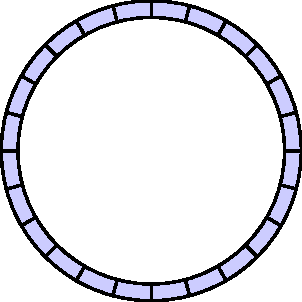
\includegraphics[width=.3\textwidth]{fig_circularList.pdf}
	  \caption{Condição de contorno periódica em um reticulado unidimensional formando um anel.}
	  \label{fig:anel}
	\end{figure}

	\begin{figure}[h!]
	  \centering
  	  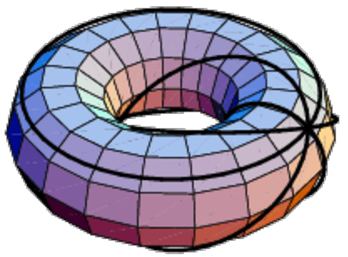
\includegraphics{fig_toro.pdf}
	  \caption{Condição de contorno periódica em um reticulado bidimensional formando um toroide.}
	  \label{fig:toro}
	\end{figure}

%TODO >>>>>>>>>>>>>>>>> Introduzir notação matemática aqui
%Estados; regras locais; e raio
As células de um autômato celular podem apresentar $k$ estados. O valor desses estados é representado ou por cores ou por valores inteiros no intervalo $[0, k-1]$. O estado de uma célula pode ser modificado pelas funções locais, que são o conjunto de regras que determinam o novo valor de uma célula baseado em seu estado atual e nos estados das células adjacentes. Para que as funções locais atualizem os valores de uma célula, é necessário que um raio $r$ seja definido. Esse raio $r$ representa o número de células adjacentes que serão analisadas em cada direção pelas funções locais.

%vizinhanças
Além do raio, é preciso determinar o formato de vizinhança que será utilizada nos parâmetros da função local. Duas vizinhanças bem comuns em ACs bidimensionais são as vizinhanças de von Neumann \cite{weisstein2015b} e Moore \cite{weisstein2015c}. Na Figura \ref{fig:vVonNeumann} e na Figura \ref{fig:vMoore} são apresentadas, para raios de 0 a 3, as vizinhanças de von Neumann e Moore, respectivamente. No caso dos ACs unidimensionais, as vizinhanças são definidas apenas pelo raio $r$ e ele descreve quantas células a esquerda e direita da célula atual serão consideras pela função local.
%TODO <<<<<<<<<<<<<<<<< Introduzir notação matemática aqui

	\begin{figure}[h!]
	  \centering
	  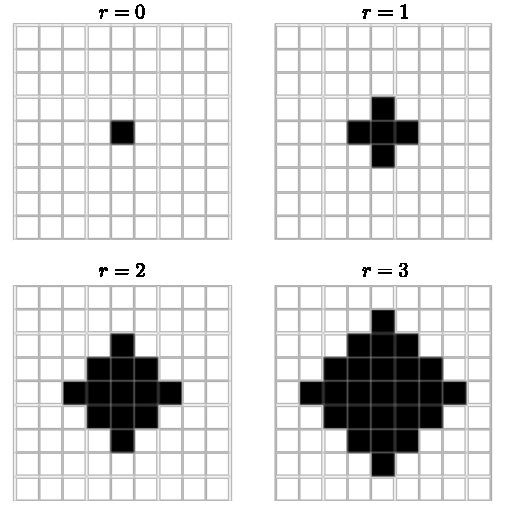
\includegraphics[width=0.45\textwidth]{fig_vVonNeumann.pdf}
	  \caption{Vizinhança de von Neumann com raio $r$ igual a 0, 1, 2 e 3. Essa foi a vizinhança utilizada nos primeiros trabalhos de von Neumann \cite{weisstein2015b}.}
	  \label{fig:vVonNeumann}
	\end{figure}

	\begin{figure}[h!]
	  \centering
  	  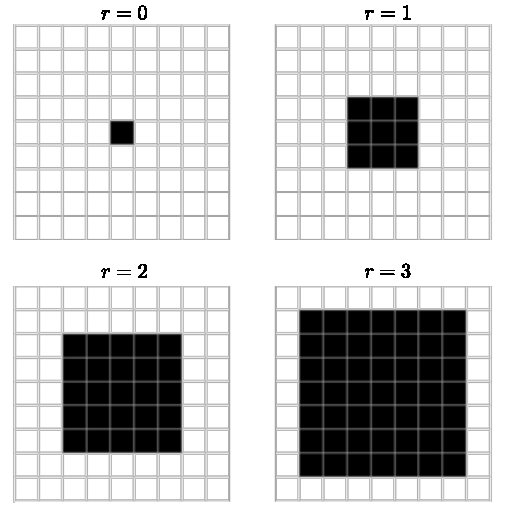
\includegraphics[width=0.45\textwidth]{fig_vMoore.pdf}
	  \caption{Vizinhança de Moore com raio $r$ igual a 0, 1, 2 e 3. Essa foi a vizinhança utilizada no jogo da vida \cite{weisstein2015c}.}
	  \label{fig:vMoore}
	\end{figure}

%Famílias de autômatos Celulares; e Autômatos Celulares Elementares.
Uma família de autômatos celulares é definida pelo raio, número de estados, tipo de vizinhança e a dimensionalidade das configurações. Autômatos celulares unidimensionais de raio $r=1$ e $k=2$ são conhecidos como a família dos autômatos celulares elementares.

Todo AC é regido por um conjunto de regras locais que determinam como ficarão as configurações no próximo passo de tempo de acordo com as configurações de vizinhança recebidas. Existem diversas maneiras de representar essas regras locais, a mais comum são as tabelas de transições. A tabela de transições é uma $n-$upla em que os elementos são todos os possíveis estados de vizinhanças de uma célula acrescentados de um estado que representa a transição que ocorrerá. A Eq. \eqref{eq:nupla} representa a $n$-upla da regra 30.
	\begin{equation}
	\begin{split}
	(((1,1,1),0),((1,1,0),0),((1,0,1),0),((1,0,0),1),\\
	((0,1,1),1),((0,1,0),1),((0,0,1),1),((0,0,0),0))
	\label{eq:nupla}
	\end{split}
	\end{equation}

Uma outra forma de representar uma tabela de transições é a forma icônica. Na forma icônica o bit $1$ é representado por um ícone na cor preta, e o bit $0$ por um ícone na cor branca. Cada uma das transições de estados é representada por um conjunto de ícones que representa a vizinhança na parte superior, e um ícone para representar o estado resultante após a transição na parte inferior. A Figura \ref{fig:repIconicaR30} mostra a representação icônica da regra 30.

	\begin{figure}[h!]
	  \centering
	  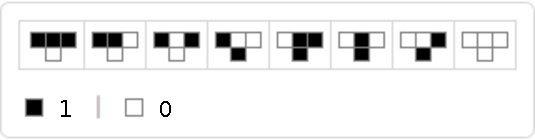
\includegraphics[width=0.6\textwidth]{fig_repIconicaR30.pdf}
	  \caption{Representação icônica da regra 30.}
	  \label{fig:repIconicaR30}
	\end{figure}

Além dessas formas de representação, ainda existe a forma $k$-ária em que, sabendo-se o valor atribuído para $k$ e $r$, elimina-se a representação das vizinhanças e deixa-se apenas as representações resultantes. Na Eq. \eqref{eq:karia} é possível ver a representação $k$-ária da regra 30. O número da regra é obtido ao se converter a representação $k$-ária para decimal. Esse número é um identificador único em família de autômatos celulares, ou seja, sempre representa apenas uma tabela de transições de estado.
	\begin{equation}
	(0,0,0,1,1,1,1,0)
	\label{eq:karia}
	\end{equation}

O número de regras de um espaço é dado pela Eq. \eqref{eq:tamFamilia}:%TODO explicar melhor
	\begin{equation}
	k^{k^{2r+1}}
	\label{eq:tamFamilia}
	\end{equation}

No espaço elementar há $2^{2^{3}} = 256$ regras. Aumentando o raio $r=2$, obtemos uma família de $2^{2^{5}} = 4.294.967.296$ regras. Para $k=3$ e $r=1$, obtém-se um espaço de ACs com $3^{3^{3}} = 7.625.597.484.987$ regras. Logo, é fácil perceber que qualquer modificação nas variáveis $k$ e $r$ geram famílias com número de regras muito grande. %TODO >>>>>>>>>>>>>>>>> Citar Algoritmos genéticos 
Famílias grandes de ACs representam um desafio na hora de encontrar ACs com propriedades específicas, já que procurar regras através de força bruta em um espaço muito grande se torna uma tarefa extremamente improdutiva. %TODO <<<<<<<<<<<<<<<<< Citar Algoritmos genéticos

Para contornar esse problema, é comum utilizar algumas propriedades estáticas para restringir as regras do espaço no qual serão feitas as buscas. Alguns exemplos de propriedades estáticas que podem auxiliar nesse ``filtro'' são o confinamento, conservabilidade de estados e conservabilidade de paridade. Todas essas propriedades são detalhadas na Seção \ref{sec:propriedadesEstaticas}.

O problema da paridade é um dos problemas que envolve fazer a ligação entre o comportamento local e o comportamento global de um autômato celular. Para o problema de paridade, nesse projeto, considera-se um AC binário, unidimensional e com condição de contorno periódica. Se uma configuração inicial contiver um número ímpar de estados com valor 1, o AC deve convergir para uma configuração global onde toda as células estejam preenchidas com 1, caso contrário, ele deve convergir para todos os estados com o valor 0. Há um problema nessa definição para  reticulado de tamanho par, pois uma configuração inicial com todos os células apresentando o estado $1$ teria que convergir para uma configuração com todos os estados apresentando o valor $0$, e o contrario também ocorreria. Desta forma o AC nunca se estabilizaria, como pede o problema. Devido essa questão, pode-se dizer que as regras que solucionam o problema de paridade em ACs são \textit{perfeitas} se eles resolverem o problema de paridade em qualquer configuração inicial arbitrária para ACs de tamanho ímpar \cite{Betel2013}. Ainda em relação ao problema de paridade, Betel, De Oliveira e Flocchini (\citeyear{Betel2013}) descrevem duas propriedades básicas: se $f$ é a regra local que resolve o problema de paridade, então $f(0, \dots, 0) = 0$ e $f(1, \dots, 1) = 1$. A segunda propriedade define que para uma regra preservar a configuração de paridade ela deve apresentar número par de transições ativas. Em outras palavras, toda aplicação da regra deve levar a uma nova configuração com a mesma paridade.

Procurar uma regra que resolva o problema de paridade em autômatos celulares unidimensionais de raio 3, por exemplo, por meio de buscas por força bruta acarretaria em testar $2^{128}$ regras. Uma maneira de facilitar essa busca é restringir as regras através propriedades estáticas, mas é necessário uma forma de representar essas propriedades e até mesmo aplicar operações como intersecção e diferença entre elas. Nesse ponto que os \textit{templates} apresentam-se de uma forma interessante e útil para representar conjuntos de regras com determinada propriedade. Templates de ACs são uma generalização das tabelas de transições que permitem representar espaços inteiros de ACs \cite{Verardo2014}.%Explicar porque o raio 3. vide p. 10

%!TEX root = qualificacao.tex
\section{TEMPLATES}
\label{sec:templates}

\textit{Templates} de autômatos celulares são uma generalização de tabelas de transições capaz de representar famílias de autômatos celulares. Os templates foram criados por De Oliveira e Verardo (\citeyear{deOliveira2014}) e implementada como um algoritmo na linguagem do software \textit{Wolfram Mathematica} \cite{woframMathematica10}, atualmente disponíveis na biblioteca \textit{open source CATemplates} \cite{CATemplates} no GitHub.

Formalmente, um \textit{template} é uma $n$-upla formada por $k^{2r+1}$ itens, e cada item $i$ representa uma função $g_i(x_0,x_1,\dots,x_{k^{2r+1}-1})$. As variáveis $x_i$ podem assumir qualquer estado entre 0 e $k-1$, logo no caso binário $x_i$ pode assumir os valores 0 e 1. É possível limitar os valores possíveis de $x_i$ através da notação $x_i \in C$, onde $C$ é um conjunto representando os possíveis valores de $x_i$. Entretanto vale frisar que no caso binário não tem lógica implementar uma notação como $x_i \in {1}$ ou $x_i \in {0}$ pois os templates também aceitam constante, sendo essas notações equivalente à apenas as constantes $1$ e $0$, respectivamente.

Exemplificando, dado um template $T_1 = (1,1,1,1,1-x_1,x_2,x_1,0)$, ele representará todas as regras que tenham na posição 0 (sempre da direita pra esquerda) o estado 0, nas posições 4, 5, 6 e 7 o estado 1, nas posições 1 e 2 qualquer estado no intervalo $[0,k-1]$ e na posição 3 o estado complementar ao valor da posição 1. Perceba que o tamanho da $n$-tupla é determinado pela função $k^{2r+1}$, logo no template $T_1$ os únicos valores inteiros possíveis para $k$ e $r$ são 2 e 1 respectivamente. Portanto $T_1$ representará um subespaço dos ACs elementares.

Deste modo o template $T_1$ representa o conjunto de autômatos celulares elementares $\{(1,1,1,1,1,0,0,0),(1,1,1,1,0,0,1,0),(1,1,1,1,1,1,0,0),(1,1,1,1,0,1,1,0)\}$, ou em sua forma decimal $\{248,242,252,246\}$.

Cada template tem um número de substituições máximo igual a $k^m$, sendo o $m$ o número de variáveis livres. O maior template possível de uma família de ACs é o \textit{template base}, em que todas as variáveis são livres. O menor é o \textit{template constante}, em que não há variáveis livres, logo representa apenas uma regra. As $8$-uplas representada pela Eq. \eqref{eq:templateConstante} representa um template constante que pode ser associado apenas a regra 30. 
\begin{equation}
(0,0,0,1,1,1,1,0)
\label{eq:templateConstante}
\end{equation}

Já a $8$-uplas, apresentada na Eq. \eqref{eq:templateBase}, representa um template base que está associado a todas as 256 regras do espaço elementar já que, para $m = 8$, temos $2^m = 256 $.
\begin{equation}
(x_7,x_6,x_5,x_4,x_3,x_2,x_1,x_0)
\label{eq:templateBase}
\end{equation}

É importante enfatizar que nem sempre o número de substituições é igual a $k^m$. Isto ocorre pois algumas substituições podem originar tabelas de transições inválidas. O template $(1,1,1,1,1,x_0+x_1,x_1,x_0)$, por exemplo, não pode apresentar as substituições $x_0=1$ e $x_1=1$ ao mesmo tempo, pois isso faz com que $x_0 + x_1 \notin [0, k-1]$, invalidando assim essa substituição para $k=2$.

A representação de famílias de autômatos celulares através de templates, possibilita a utilização de templates para problemas já bem conhecidos da área de ACs. Um exemplo de problema que pode se beneficiar dos templates é o problema da paridade.

A Figura \ref{fig:parity-rule} ilustra o desenvolvimento espaço-temporal da regra BFO \cite{Betel2013} que resolve o problema de paridade para o raio 4. Nessa imagem o desenvolvimento temporal à esquerda contém, em sua configuração inicial, um número par de estados igual a 1, já na evolução temporal ilustrada à direita há um número ímpar de estados igual a 1.

\begin{figure}[h!]
\center
\subfigure[CI com número ímpar de 1s]{
\includegraphics[width=4.8cm]{regra-1-par.pdf}}
\qquad
\subfigure[CI com número par de 1s]{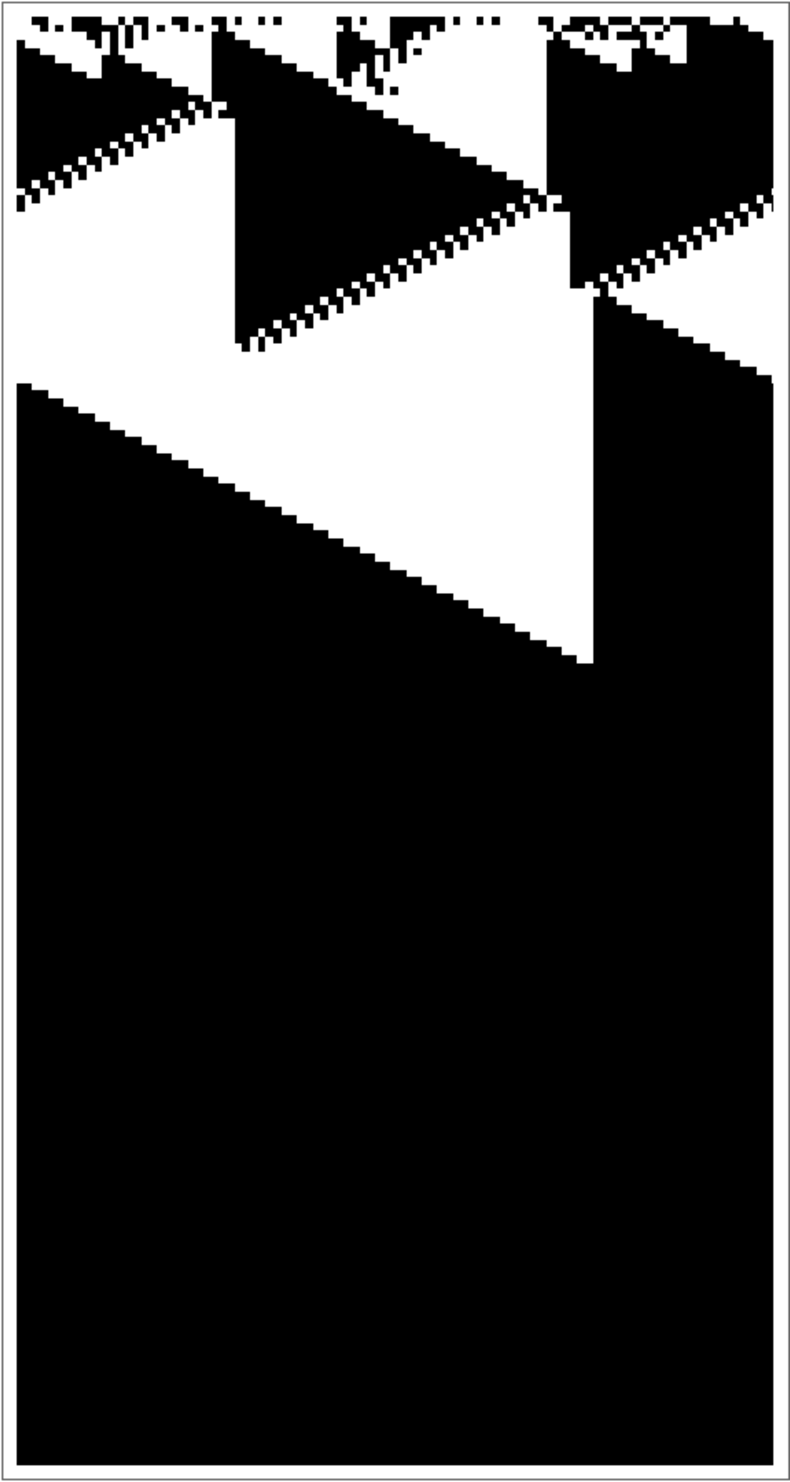
\includegraphics[width=4.8cm]{regra-1-impar.pdf}}
\caption{Desenvolvimento espaço-temporal da regra BFO, que resolve o problema de paridade para raio 4. \cite{Betel2013}}
\label{fig:parity-rule}
\end{figure}

O estudo do problema da paridade é interessante pois ajuda a compreender o impacto das interações locais nas soluções globais. Especificamente, entender a influência que o tamanho da vizinhança em autômatos celulares apresenta na computabilidade pode apresentar consequências úteis tanto para ACs como para a compreensão de sistemas emergentes complexos em geral.

Estudos feitos sobre o problema de paridade já levaram ao conhecimento de que o problema não tem solução perfeita para ACs elementares e de raio 2, todavia já foi descoberta uma regra perfeita que soluciona o problema de paridade para raio 4. Em relação aos ACs de raio 3, ainda não foi encontrada solução perfeita e há evidências empíricas desfavoráveis a uma solução para esse raio \cite{Betel2013}.

Betel, De Oliveira e Flocchini (\citeyear{Betel2013}), buscando verificar se o problema da paridade em ACs de raio 2 apresentam alguma regra que solucione o problema para qualquer configuração inicial, encontraram de forma analítica como as transações de estado de supostas regras que resolvessem o problema de paridade deveriam ser. 

Para representar como as transações de estado deveriam ser, foi utilizado grafos de \textit{De Bruijn}. Grafos de \textit{De Bruijn} são grafos cujos nós são sequências de símbolos de algum alfabeto e cujas arestas indicam as sequências em que se cruzarão \cite{weisstein2015deBruijn}. Em AC, esse tipo de grafo direcionado apresenta em suas arestas o resultado de uma transição de estado, e a vizinhança é representada no grafo pela sobreposição dos dois nós ligados pela aresta de resultado. 

%MEUTODO Talvez colocar um imagem ilustrando os grafos de \textit{De Bruijn} aqui.

Com isso, utilizando grafos de \textit{De Bruijn} foram definidas quais variáveis deveriam ser estáticas, quais deveriam ser livres e quais deveriam apresentar interdependência. Com essas definições foram definidas duas famílias de ACs. Os grafos ilustrados na Figura \ref{fig:grafosDeBruijn} e na Figura \ref{fig:grafosDeBruijn2} são os grafos desenvolvidos por Betel, De Oliveira e Flocchini (\citeyear{Betel2013}).

\begin{figure}[h!]
\centering
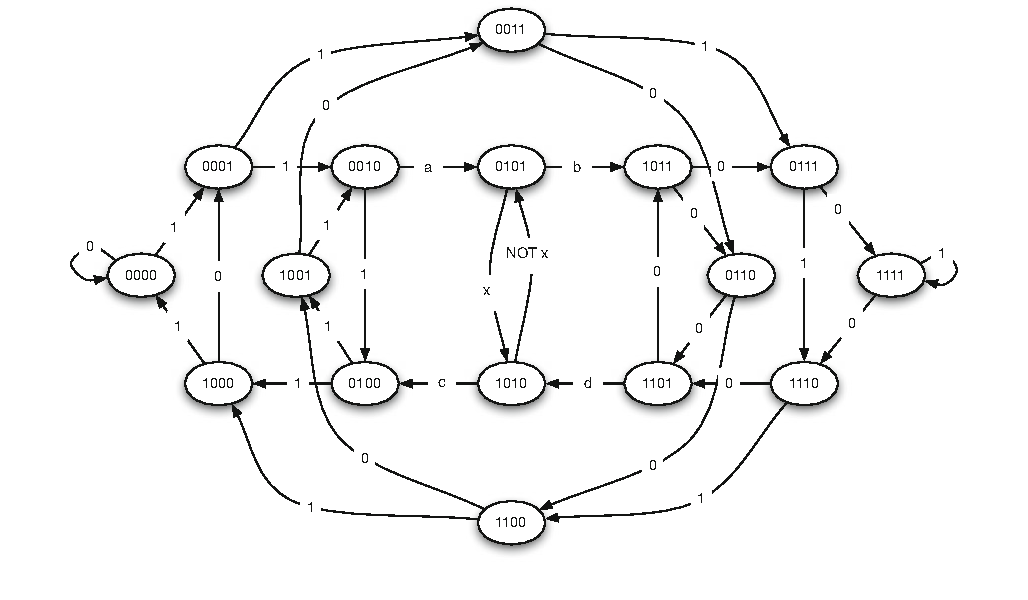
\includegraphics[width=.8\textwidth]{grafo1.pdf}
\caption{Grafo de De Bruijn representando regras que possivelmente solucionem o problema de paridade. \cite{Betel2013}}
\label{fig:grafosDeBruijn}
\end{figure}

Ambos os grafos apresentam arestas contendo as variáveis livres $a, b, c, d \text{ e } x$ e uma interdependência, em que uma transição de estado deve ter o valor oposto à variável $x$. A única diferença entre os dois grafos está nas arestas contendo variáveis estáticas.

\begin{figure}[h!]
\centering
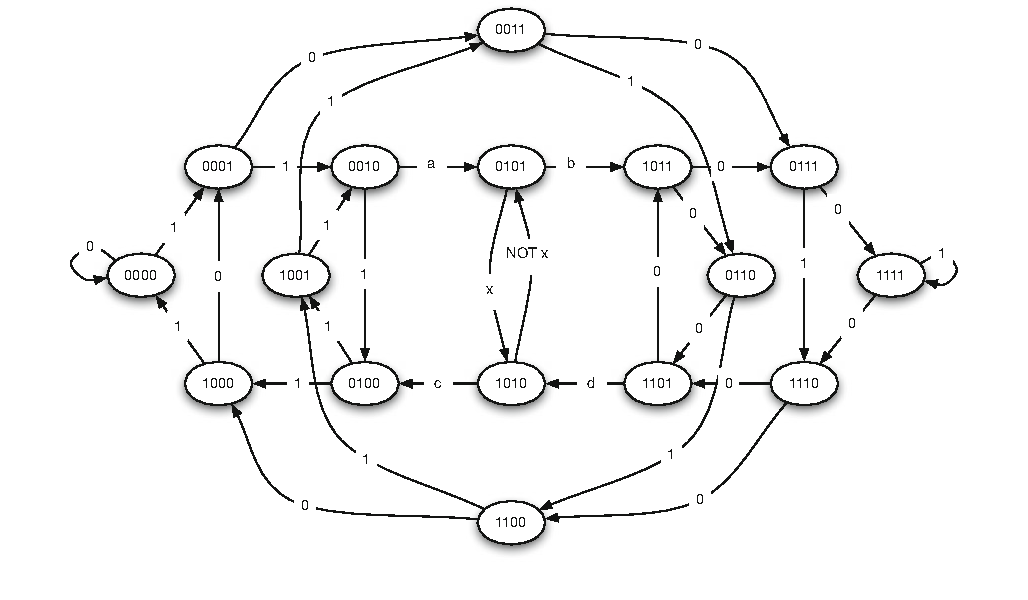
\includegraphics[width=1\textwidth]{grafo2.pdf}
\caption{Outro grafo de De Bruijn representando regras que possivelmente solucionem o problema de paridade.\cite{Betel2013}}
\label{fig:grafosDeBruijn2}
\end{figure}

Ao utilizar os grafos de \textit{De Bruijn} fixando algumas transições de estado a família de ACs em que se procurava as regras que solucionavam o problema de paridade foi restringida para apenas 64 regras. Ao se restringir o espaço de busca, antes composto por $2^{32}$ regras, as regras puderam ser estudadas em mais detalhes até que falhassem. Entretanto, conforme mostrado em \cite{Verardo2014}, a representação desse espaço de 64 regras pode ser equivalentemente representado por meio de \textit{templates}. O template da Eq. \eqref{eq:templateParidade1} representa o mesmo espaço que a Figura \ref{fig:grafosDeBruijn}, já o template da Eq. \eqref{eq:templateParidade2} é equivalente a Figura \ref{fig:grafosDeBruijn2}. Ambos templates apresentam raio $r=2$ e apenas dois estados.
\begin{equation}
\left(0,1,1,1,1,x_{26},0,1,1,1,1-x_{10},x_{20},0,0,1,0,1,0,1,0,x_{11},x_{10},0,0,1,0,x_5,0,1,0,0,1\right)
\label{eq:templateParidade1}
\end{equation}
\begin{equation}
\left(0,1,1,0,1,x_{26},1,0,1,1,1-x_{10},x_{20},0,1,1,0,1,0,1,1,x_{11},x_{10},0,0,1,0,x_5,0,0,0,0,1\right)
\label{eq:templateParidade2}
\end{equation}


\newpage\newpage
\subsection{Expansão de Templates}
Expansão é o processo no qual se obtêm todas as tabelas de transição $R_k$ associadas a um template $T$.
A operação de expansão foi apresentada por \citeonline{Verardo2014} e foi descrita em mais detalhes da seguinte maneira:

\begin{equation}
E(T)=R_k
\end{equation}

A operação de expansão pode ser dividida em dois passos, em que o primeiro consiste em efetuar todas as $i$ substituições de variáveis, sendo que $i$ pertence ao intervalo discreto $[0,k^m-1]$. Considere como exemplo o template $T_1 = (1,1,1,1,1-x_1,x_2,x_1,0)$, o primeiro passo do processo de expansão consiste em encontrar as tabelas $k$-árias resultantes das combinações possíveis das substituições de $x_1$ e $x_2$, conforme pode ser melhor visualizado na Tabela \ref{tab:expansionProcess}.

\begin{table}[h!]
\centering
\caption{Processo de expansão}
{
	\vspace{0.3cm}
	\begin{tabular}{cccc}
	\hline
	$i$ & $x_2$ & $x_1$ & tabela $k$-ária resultante \\
	\hline
	0	&	0	&	0	&	(1,1,1,1,1,0,0,0)	\\
	1	&	0	&	1	&	(1,1,1,1,1,1,0,0)	\\
	2	&	1	&	0	&	(1,1,1,1,0,0,1,0)	\\
	3	&	1	&	1	&	(1,1,1,1,0,1,1,0)	\\
	\hline
	\end{tabular}
}
\label{tab:expansionProcess}
\end{table}

O segundo passo da operação de expansão é eliminar as tabelas $k$-ária inválidas. No caso do template $T_1$ todas as tabelas resultantes eram válidas, mas nem sempre isso ocorre. No template $T_2 = (1,1,1,1,1,x_0+x_1,x_1,x_0)$, por exemplo, a substituição $x_0 = 1$ e $x_1 = 1$ resulta numa tabela $k$-ária inválida pois a terceira posição apresenta um estado com um valor fora do interval $[0,k-1]$, para $k=2$. A Tabela \ref{tab:invalideExpansion} evidência melhor essa substituição inválida.

\begin{table}[h!]
\centering
\caption{Processo de expansão}
{
	\vspace{0.3cm}
	\begin{tabular}{cccc}
	\hline
	$i$ & $x_1$ & $x_0$ & tabela $k$-ária resultante \\
	\hline
	0	&	0	&	0	&	(1,1,1,1,1,0,0,0)	\\
	1	&	0	&	1	&	(1,1,1,1,1,1,0,1)	\\
	2	&	1	&	0	&	(1,1,1,1,1,1,1,0)	\\
	3	&	1	&	1	&	(1,1,1,1,1,2,1,1)	\\
	\hline
	\end{tabular}
}
\label{tab:invalideExpansion}
\end{table}

Ainda há outra maneira em que templates resultam em substituições inválidas, sendo uma delas através da utilização da notação restrição por conjuntos. Considere o templates $T_3 = (2,2,2,2,2,2,2,2,x_0\in \{0,1\})$ da família de $k=3$ e $r=0{,}5$. %TODO Explicar raio 0,5
A substituição obtida para $i = 2$ seria inválida pois nesse caso $x_0 = 2$ e $2 \notin \{0,1\}$. A Tabela \ref{tab:invalideExpansion2} evidencia melhor esse processo.

\begin{table}[h!]
\centering
\caption{Processo de expansão}
{
	\vspace{0.3cm}
	\begin{tabular}{cccc}
	\hline
	$i$ & $x_0$ & tabela $k$-ária resultante \\
	\hline
	0	&	0	&	(2,2,2,2,2,2,2,2,0)	\\
	1	&	1	&	(2,2,2,2,2,2,2,2,1)	\\
	2	&	2	&	(2,2,2,2,2,2,2,2,2)	\\
	\hline
	\end{tabular}
}
\label{tab:invalideExpansion2}
\end{table}

A existência de regras inválidas são os responsáveis por templates que representem um conjunto de regras menores que $k^m$. Essa possibilidade é bastante útil para os templates de regras conservativas e regras confinadas.

O valor de $i$ sempre representa apenas uma substituição possível para as variáveis livres de um templates. Isso ocorre pois $i$ é a representação decimal da conversão $k$-ária das concatenações dos valores das variáveis livres em ordem decrescente. Exemplificando, considere o templates $T_3 = (2,2,2,2,2,2,2,x_1,x_0\in \{0,1\})$ para $k=3$. O valor de $i=5$ será convertido pelo processo de expansão obtendo-se assim o seu equivalente na base ternária $(1,2)$ e então cada um dos dígitos é atribuído a uma variável, resultando assim no conjunto de substituições ${x_0=2,x_1=1}$.

A forma com que o valor de $i$ representa apenas uma expansão permite possibilidade de se obter a $i$-ésima expansão de um template. Essa propriedade é relevante devido ao fato da expansão ser uma operação potencialmente custosa, e a possibilidade de ser realizar a $i$-ésima expansão de um template facilita e permite o paralelismo.

\newpage\newpage
\subsection{Intersecção de Templates}
Intersecção é o processo no qual, dado dois templates $T_1$ e $T_2$, se obtêm um template que represente o conjunto $R_k$. O conjunto $R_k$ representa todas as regras pertencentes aos dois templates recebidos como parâmetro. É necessário que os dois templates recebidos como parâmetro pertençam ao mesmo espaço. A operação de intersecção foi descrita por \citeonline{Verardo2014} e mostrada em mais detalhes da seguinte maneira:

\begin{equation}
I(T_1,T_2)=T_3 \Leftrightarrow E(T_3) = E(T_1) \cap E(T_2)
\end{equation}

A operação de intersecção, assim como a de expansão, também é efetuada em duas etapas. Na primeira etapa iguala-se os dois templates e assim se obtêm um sistema de equações. Esse sistema de equações é então passado como argumento para a função Solve, função essa nativa da \textit{Wolfram Language} \cite{woframMathematica10}. A função Solve retorna então os relacionamentos entre as variáveis, que ao serem aplicados aos templates recebidos, retorna dois template equivalente, bastando escolher um que será o template de intersecção. No caso dos templates não apresentarem intersecção, a função Solve não retornará solução.

Para melhor compreensão, considere os templates $T_1 = (x_7,x_3,1-x_4,x_4,x_3,x_2,2,x_0)$ e $T_2 = (x_7,1,x_5,0,x_3,x_2,2,2)$, ambos com $r=0{,}5$ e $k=3$. Esse templates serão transformados em um sistema de equações como demonstrado na Eq. \eqref{eq:interseccao}.

\begin{equation}
\left\{\begin{matrix}
x_7   & = & x_7 \\ 
x_3   & = & 1 \\ 
1-x_4 & = & x_5    \\ 
x_4   & = & 0    \\ 
x_3   & = & x_3    \\ 
x_2   & = & x_2   \\ 
2     & = & 2   \\ 
x_0   & = & 2
\end{matrix}\right.
\label{eq:interseccao}
\end{equation}

Esse sistema de equações é passado então como argumento para a função Solve, que por sua vez retorna um conjunto solução $S$, que nesse exemplo é $S = \{x_0 = 2, x_3 = 1, x_4 = 0, x_5 = 1 - x_4, x_6 = 0\}$. O conjunto $S$ é aplicado como um conjunto de substituições sobre os dois templates recebidos como parâmetro, que em caso de templates sem restrição de variáveis sempre retorna o mesmo template. Neste exemplo, após aplicada as substituições do conjunto de soluções $S$, obtêm-se como resultado o template $T_3 = (x_7, 1, 1, 0, 1, x_2, 2, 2)$.

A segunda etapa do algoritmo apenas é aplicada para templates com alguma restrição de variável. Essa etapa consiste em extrair as expressões que estabelecem as restrições, e através delas obter um segundo sistema de equações. A solução desse sistema ou pode ser vazia, expressando assim que os templates não tem intersecção, ou pode indicar os valores que as variáveis com restrição podem assumir.

Para exemplificar essa segunda etapa, considere os templates $T_{r1} = (x_7 \in \{0,1,2\},x_3,1-x_4,x_4,x_3,x_2 \in \{1,2\},2,x_0)$ e $T_{r2} = (x_7 \in \{0,1\},1,x_5,0,x_3,x_2 \in \{1\},2,2)$. A primeira etapa ocorre normalmente, entretanto, quando as substituições do conjunto $S$ forem aplicadas nos templates recebidos, não será mais obtido templates iguais. Nesse caso o conjunto de templates obtidos será $\{(x_7 \in \{0,1,2\}, 1, 1, 0, 1, x_2 \in \{1,2\}, 2, 2), (x_7 \in \{0,1\}, 1, 1, 0, 1, x_2 \in \{1\}, 2, 2)\}$. Na sequencia o algoritmo faz a extração das expressões de restrição de variáveis e obtêm o conjunto $\{x_7 \in \{0,1\}, x_2 \in \{1,2\}, x_2 \in \{1\} \}$. Esse conjunto é então convertido para o sistema de equações representadas pela Eq. \eqref{eq:interseccaoRestrita}.

\begin{equation}
\left\{\begin{matrix}
x_7	  = 0 	& \vee &	x_7	=	1 & \vee &	x_7	= 2	\\ 
x_7   = 0 	& \vee &	x_7	=	1					\\ 
x_2   = 1 	& \vee &	x_2	=	2					\\ 
x_2	  =	1											\\ 
\end{matrix}\right.
\label{eq:interseccaoRestrita}
\end{equation}

Esse sistema de equações é então passado como argumento para a função Solve, que retorna seu conjunto solução. Por fim o algoritmo usa o conjunto solução retornado para remover as restrições da variável $x_2$, transformando-a no valor $1$, e restringi a variável $x_7$ apenas ao conjunto $\{0,1\}$. O template de intersecção gerado por todo esse processo é representado pela Eq. \eqref{eq:templateIntescecao}.

\begin{equation}
T_{r3} = (x_7 \in \{0,1\}, x_3, 1-x_4, x_4, x_3, 1, 2, x_0)
\label{eq:templateIntescecao}
\end{equation}

Vale frisar que o template $T_{r2}$ também poderia ser representado substituindo a variável $x_2$ e seu conjunto de restrição $\{1\}$ apenas pelo valor constante $1$, como mostrado a seguir: $T_{r2} = (x_7 \in \{0,1\}, 1, x_5, 0, x_3, 1, 2, 2)$. Esse tipo de mudança é sempre preterido pois variáveis a mais acarretam em mais processamento.

No caso binário, ou seja $k = 2$, a notação de restrição nunca é necessária visto que ou a restrição terá apenas um valor factível, sendo preferível que essa variável e sua restrição sejam substituídas por um valor constante, ou a variável poderá assumir qualquer estado sendo assim, por definição, uma variável livre.

%!TEX root = qualificacao.tex
\section[REPRESENTAÇÃO DE PROPRIEDADES ESTÁTICAS POR MEIO DE TEMPLATES]{REPRESENTAÇÃO DE PROPRIEDADES \\ ESTÁTICAS POR MEIO DE TEMPLATES}
\label{sec:propriedadesEstaticas}

Em ACs, propriedades estáticas são propriedades computadas com base nas tabelas de transição. Essas propriedades permitem prever determinados comportamentos de um ACs sem consultar sua evolução espaço-temporal. 

Esta seção descreverá algumas propriedades estáticas e os algoritmos geradores de templates que as representam. Todos algoritmos explicados estão implementados na biblioteca \textit{CATemplates} \cite{CATemplates}.

\subsection{Conservabilidade de Estados e Conservabilidade de Paridade}
Conservabilidade de estados é uma propriedade estática que determina que a soma dos estados de um determinado autômato celular não deve se alterar durante a evolução espaço-temporal, independente da configuração inicial passada.

De acordo com Boccara e Fukś (\citeyear{boccara2002}), um AC é conservativo quando cada uma de suas regras locais $f$ de vizinhança $(\alpha_0,\alpha_1, \dots, \alpha_{n-1})$ respeita as condições descritas na Eq. \eqref{eq:conservativeCA}.

\begin{equation}
\begin{split}
f(\alpha_0,\alpha_1, \dots,\alpha_{n-1}) = \alpha_0 + (\sum_{i=0}^{n-2}f(0_0,0_1, \dots,0_i,\alpha_1,\alpha_2, \dots,\alpha_{n-1}) \\- f(0_0,0_1, \dots,0_i,\alpha_0,\alpha_1, \dots,\alpha_{n-i-1}))
\label{eq:conservativeCA}
\end{split}
\end{equation}

Para exemplificar, considere a regra 204 do espaço elementar. Por meio da condição mostrada na Eq. \eqref{eq:conservativeCA}, será provado que essa regra é conservativa, já que satisfaz a condição. A Eq. \eqref{eq:ruleTable204} representa a tabela de transições da regra 204.

\begin{equation}
\begin{split}
(((1,1,1),1),((1,1,0),1),\\((1,0,1),0),((1,0,0),0),\\((0,1,1),1),((0,1,0),1),\\((0,0,1),0),((0,0,0),0))
\label{eq:ruleTable204}
\end{split}
\end{equation}

Como demonstra \citeonline{Verardo2014}, a aplicação das condições da Eq. \eqref{eq:conservativeCA} nas tabelas de transições de ACs do espaço elementar, sempre resultará no sistema descrito pela Eq. \eqref{eq:conservativeLinearSystem}.

\begin{equation}
\left\{\begin{matrix}
 f(0,0,0) = 0 + (f(0,0,0) - f(0,0,0)) + (f(0,0,0) - f(0,0,0))\\ 
 f(0,0,1) = 0 + (f(0,0,1) - f(0,0,0)) + (f(0,0,0) - f(0,0,0))\\ 
 f(0,1,0) = 0 + (f(0,1,0) - f(0,0,1)) + (f(0,0,1) - f(0,0,0))\\ 
 f(0,1,1) = 0 + (f(0,1,1) - f(0,0,1)) + (f(0,0,1) - f(0,0,0))\\ 
 f(1,0,0) = 1 + (f(0,0,0) - f(0,1,0)) + (f(0,0,0) - f(0,0,1))\\ 
 f(1,0,1) = 1 + (f(0,0,1) - f(0,1,0)) + (f(0,0,0) - f(0,0,1))\\ 
 f(1,1,0) = 1 + (f(0,1,0) - f(0,1,1)) + (f(0,0,1) - f(0,0,1))\\ 
 f(1,1,1) = 1 + (f(0,1,1) - f(0,1,1)) + (f(0,0,1) - f(0,0,1))
\end{matrix}\right.
\label{eq:conservativeLinearSystem}
\end{equation}

A Eq. \eqref{eq:conservativeLinearSystem} simplificada é representada pela Eq. \eqref{eq:conservativeLinearSystem2}.

\begin{equation}
\left\{\begin{matrix}
 f(0,0,0) & = & 0 		& &\\ 
 f(0,0,1) & = & f(0,0,1)& & \\ 
 f(0,1,0) & = & f(0,1,0)& & \\ 
 f(0,1,1) & = & f(0,1,1)& & \\ 
 f(1,0,0) & = & 1 - f(0,0,1) - f(0,1,0) \\ 
 f(1,0,1) & = & 1 - f(0,1,0) \\ 
 f(1,1,0) & = & 1 + (f(0,1,0) - f(0,1,1))\\ 
 f(1,1,1) & = & 1 & &
\end{matrix}\right.
\label{eq:conservativeLinearSystem2}
\end{equation}

Excluindo-se as condições tautológicas do sistema e atribuindo os valores das funções locais $f$ conforme a tabela de transições da regra 204, é obtido o sistema descrito pela Eq. \eqref{eq:conservativeAC204}. Esse sistema, ao não apresentar condições contraditórias ou falsas, prova que a regra 204 é conservativa.

\begin{equation}
\left\{\begin{matrix}
 0 & = & 0 \\ 
 0 & = & 1 - 0 - 1 \\ 
 0 & = & 1 - 1 \\ 
 1 & = & 1 + (1 - 1)\\ 
 1 & = & 1 
\end{matrix}\right.
\label{eq:conservativeAC204}
\end{equation}

O algoritmo que gera templates que representam regras conservativas, criado por De Oliveira e Verardo (\citeyear{deOliveira2014}), primeiramente recebe as variáveis $k$ e $r$ definindo assim a família das regras que serão geradas. Em seguida, cria todas as vizinhanças do espaço com exceção das vizinhanças que geram tautologias. E após esses passos, aplica as condições de Boccara e Fukś (\citeyear{boccara2002}). Para se excluir as vizinhanças que geram tautologias, basta excluir as vizinhanças que começam com 0 mas não sejam compostas apenas por 0 \cite{Schranko2010}.

Para exemplificar o funcionamento do algoritmo, considere um espaço com $k=2$ e $r=1$. Primeiramente o algoritmo obterá o conjunto das vizinhanças que não geram regras tautológicas, portanto será obtido o conjunto $\{(1,1,1),(1,1,0),(1,0,1),(1,0,0),(0,0,0)\}$. Então é criado o sistema de equações \eqref{eq:conservativeLinearSystem3}, baseado nas condições de Boccara e Fukś (\citeyear{boccara2002}).

\begin{equation}
\left\{\begin{matrix}
 x_0 & = & 0\\ 
 x_4 & = & 1 +2x_0 -x_1 -x_2\\ 
 x_5 & = & 1 +x_0 -x_2\\
 x_6 & = & 1 +x_2 -x_3\\ 
 x_7 & = & 1
\end{matrix}\right.
\label{eq:conservativeLinearSystem3}
\end{equation}

Por fim o algoritmo utiliza a função Solve do \textit{Wolfram Mathematica} para simplificar o sistema e utiliza o conjunto solução retornado pela função Solve como regras de substituições. Essas regras de substituições são aplicadas no template base, gerando assim o template das regras conservativas. O template gerado pode ser observado na Eq. \eqref{eq:conservativeTemplate}, e sua expansão gera as cinco regras conservativas do espaço elementar, após eliminadas as regras inválidas.

\begin{equation}
(1,x_2-x_3+1,1-x_2,-x_1-x_2+1,x_3,x_2,x_1,0)
\label{eq:conservativeTemplate}
\end{equation}

O processo de gerar regras conservativas de paridade é bem parecido. Porém as condições estabelecidas por Boccara e Fukś (\citeyear{boccara2002}) são ligeiramente modificadas em relação a Eq. \eqref{eq:conservativeCA}, de forma que cada uma das funções locais deve respeitar agora as condições da Eq. \eqref{eq:parityConservativeCA}.

\begin{equation}
\begin{split}
f(\alpha_0,\alpha_1, \dots,\alpha_{n-1}) \equiv \alpha_0 + (\sum_{i=0}^{n-2}f(0_0,0_1, \dots,0_i,\alpha_1,\alpha_2, \dots,\alpha_{n-1}) \\- f(0_0,0_1, \dots,0_i,\alpha_0,\alpha_1, \dots,\alpha_{n-i-1})) \; (mod 2)  
\label{eq:parityConservativeCA}
\end{split}
\end{equation}

A biblioteca \textit{CATemplates} já tem implementado o algoritmo gerador de templates de regras conservativas de paridade, e conforme será mostrado posteriormente, esse algoritmo pode ser de suma importância na busca de uma solução para o problema de paridade.





\subsection{Confinamento}
Os autômatos celulares confinados, ou \textit{captive} em Inglês, são uma classe de AC que se baseiam em uma caracterização de suas funções locais que não adotem estados definidos em qualquer estrutura externa à vizinhança \cite{theyssier2004captive}. 

\citeonline{theyssier2004captive} formalmente define que dado a função local $f$ de um AC para a vizinhança $(\alpha_0, \dots, \alpha_{2r})$, sendo o $r$ o raio, um AC é considerado confinado se respeitar a condição descrita na Eq. \eqref{eq:captiveAC}.

\begin{equation}
f((\alpha_0, \dots, \alpha_{2r})) = \beta, \beta \in \{\alpha_0, \dots, \alpha_{2r}\}
\label{eq:captiveAC}
\end{equation}

Essa propriedade pode ser facilmente representada através de templates. Para isto, basta restringir as variáveis a um conjunto de valores presentes na vizinhança correspondente. A biblioteca \textit{open source CATemplates} já apresenta um algoritmo que gera as regras confinadas. Esse algoritmo recebe como parâmetro os argumentos $k$ e $r$. Após isso, gera as vizinhanças do espaço e verifica em cada uma das vizinhanças os estados que elas têm. Caso a vizinhança tenha todos os estados do intervalo $[0, k-1]$ essa posição terá uma variável livre no template. Caso a vizinhança tenha apenas um estado a posição correspondente no template assume um valor fixo. Por fim, caso a vizinhança apresente mais de um estado, mas não todos, a posição correspondente do template apresentará uma variável restritas mediante expressões $x_i \in C$.

É trivial perceber que qualquer AC binário que tenha as funções locais $f((0_0, 0_1,\dots, 0_{2r})) = 0$ e $f((1_0, 1_,1\dots, 1_{2r})) = 1$ é caracterizado como um AC confinado. A Eq. \eqref{eq:captiveTemplateACE} representa o template de todas as regras confinadas do espaço elementar e a Eq. \eqref{eq:captiveTemplateR05} representa a família de $k=2$ e $r=0,5$.
\begin{equation}
(1,x_6,x_5,x_4,x_3,x_2,x_1,0)
\label{eq:captiveTemplateACE}
\end{equation}

\begin{equation}
(1,x_2,x_1,0)
\label{eq:captiveTemplateR05}
\end{equation}

Por fim, a Eq. \eqref{eq:captiveTemplateK3} representa a família dos autômatos celulares confinados de $r=1$ e três estados.

\begin{equation}
\begin{split}
(2, x_{25} \in \{1,2\}, x_{24} \in \{0,2\}, x_{23} \in \{1,2\}, x_{22} \in \{1,2\}, x_{21}, x_{20} \in \{0,2\}, x_{19}, x_{18} \in \{0,2\}, \\
x_{17} \in \{1,2\}, x_{16} \in \{1,2\}, x_{15}, x_{14} \in \{1,2\},1, x_{12} \in \{0,1\}, x_{11}, x_{10} \in \{0,1\}, x_9 \in \{0,1\}, \\
x_8 \in \{0,2\}, x_7, x_6 \in \{0,2\}, x_5, x_4 \in \{0,1\}, x_3 \in \{0,1\}, x_2 \in \{0,2\}, x_1 \in \{0,1\}, 0)
\label{eq:captiveTemplateK3}
\end{split}
\end{equation}

\subsection{Simetria Interna}
Para entender a propriedade de simetria interna faz-se necessário compreender o funcionamento das transformações de regras e classes de equivalência dinâmica. As explicações a seguir são válidas para regras binárias pois o algoritmo hoje implementado no CATemplates é para regras binárias, apesar de ser possível sua generalização para $k$ estados.

Dado uma tabela de transições de um AC, existem três transformações que podem ser empregadas e que resultam em ACs com comportamentos dinâmicos equivalentes: \textit{reflexão}, \textit{conjugação} e \textit{composição}. A reflexão é a transformação obtida ao refletir os bits das vizinhanças da tabela. A conjugação é obtida ao inverter todos os estados das células da tabela de transições. Já a composição é a transformação obtida ao se efetuar a reflexão e a conjugação, independente da ordem.

Essas transformações podem ser aplicadas tanto a vizinhança, como também podem ser aplicadas a toda a tabela de transições. Para aplicar uma transformação a toda uma tabela, basta aplicá-la a cada uma das vizinhanças da tabela. Uma tabela, transição ou vizinhança é chamada de invariante a uma transformação caso essa transformação, quando aplicada a ela, não promova nenhum efeito. Um exemplo de vizinhança invariante por reflexão é a vizinhança $(1,0,1)$. A vizinhança $(1,0,1)$ após aplicada a transformação por reflexão, continua sendo a mesma vizinhança.

Para exemplificar essas transformações e as equivalências dinâmicas considere a tabela de transição da regra 60, ilustrada pela Figura \ref{fig:table60}. Ao se aplicar a transformação por reflexão na regra 60 obtemos a regra 102 do espaço elementar, ilustrada pela Figura \ref{fig:table102}.

	\begin{figure}[h!]
	  \centering
	  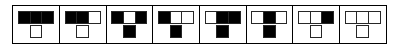
\includegraphics[width=.7\textwidth]{fig_ruleIcon60.png}
	  \caption{Tabela de transições da regra 60 do espaço elementar.}
	  \label{fig:table60}
	\end{figure}

	\begin{figure}[h!]
	  \centering
	  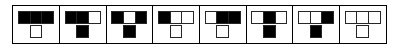
\includegraphics[width=.7\textwidth]{fig_ruleIcon102.png}
	  \caption{Tabela de transições da regra 102 do espaço elementar, obtida através da transformação de reflexão aplicada na tabela de transições da regra 60.}
	  \label{fig:table102}
	\end{figure}

Ao se aplicar a transformação por conjugação na regra 60 obtemos a regra 195 do espaço elementar, conforme ilustrado na Figura \ref{fig:table195}. E por fim, ao se aplicar a transformação por composição de reflexão e conjugação na regra 60 obtemos a regra 153 do espaço elementar, conforme ilustrado na Figura \ref{fig:table153}.

	\begin{figure}[h!]
	  \centering
	  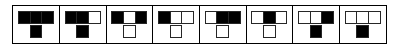
\includegraphics[width=.7\textwidth]{fig_ruleIcon195.png}
	  \caption{Tabela de transições da regra 195 do espaço elementar, obtida através da transformação de conjugação aplicada na tabela de transições da regra 60.}
	  \label{fig:table195}
	\end{figure}

	\begin{figure}[h!]
	  \centering
	  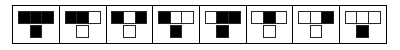
\includegraphics[width=.7\textwidth]{fig_ruleIcon153.png}
	  \caption{Tabela de transições da regra 153 do espaço elementar, obtida através da transformação de composição aplicada na tabela de transições da regra 60.}
	  \label{fig:table153}
	\end{figure}

Tanto a regra 60, como as regras 102, 153 e 195 pertencem a mesma classe de equivalência dinâmica. Uma forma interessante de entender o porquê é analisando a evolução espaço-temporal dessas regras, ilustrada pela Figura \ref{fig:dynamicEquivalecy}.

	\begin{figure}[h!]
	  \centering
	  \def\svgscale{0.63}
	  \import{../img/}{fig_ruleEquivalence60.pdf_tex}
	  \caption{Evolução espaço-temporal das regras pertencente à mesma classe dinâmica da regra 60.}
	  \label{fig:dynamicEquivalecy}
	\end{figure}

Tendo em vista as tabelas de transições obtidas por meio das transformações, é possível saber quão simétrica é uma regra, ou em outras palavras, qual a simetria interna de uma regra em relação a uma determinada transformação. A simetria interna pode ser representada pelo número de vizinhanças que permanecem iguais após aplicada uma determinada transformação. Exemplificando, a regra 60 dos ACs elementares tem um valor de simetria interna por reflexão igual a 4, pois compartilha as transições de estado $((1,1,1),0)$, $((1,0,1),1)$, $((0,1,0),1)$ e $ ((0,0,0),0)$ com a regra resultante de sua transformação por reflexão, a regra 102. Vale notar que as vizinhanças compartilhadas são todas as vizinhanças invariantes do espaço elementar, logo pode-se dizer que a regra 60 tem a menor simetria interna possível para o espaço elementar.

Um resultado bem diferente pode ser visto ao se repetir esse mesmo processo para a regra 204, que tem o valor 8 de simetria interna para transformação por reflexão. Esse valor é máximo possível para o espaço elementar e evidencia que ao se aplicar a transformação por reflexão na regra 204 será obtida a mesma regra como resultado. Uma regra contiver máxima simetria para uma transformação é uma regra invariante.

Vale frisar que apenas transformações por reflexão apresentam vizinhanças invariantes. No caso das reflexões por conjugação e por composição isso não ocorre.

Já há implementado no CATemplates um algoritmo gerador de templates que representam regras do espaço binário com um determinado valor de simetria para uma transformação.

O algoritmo recebe como parâmetro um raio $r$, definindo assim a família de ACs que será representada, o valor de simetria interna desejado, e uma das transformações de simetria.

Para melhor representar o funcionamento do algoritmo, considere que foi passado como parâmetro um raio $r = 1$, a transformação de reflexão e a simetria interna desejada igual a 8. O primeiro passo do algoritmo será gerar todas as vizinhanças do espaço, que no nosso exemplo pode ser representado pela conjunto descrito pela Eq. \eqref{eq:neighborSetACE}
\begin{equation}
\{(1,1,1),(1,1,0),
(1,0,1),(1,0,0),
(0,1,1),(0,1,0),
(0,0,1),(0,0,0)\}
\label{eq:neighborSetACE}
\end{equation}

Após isso, a transformação escolhida, no caso reflexão, é aplicada a cada uma das vizinhanças, gerando assim o conjunto representado pela Eq. \eqref{eq:neighborSetTransformadoACE}.  
\begin{equation}
\begin{split}
\{
((1,1,1),(1,1,1)),
((1,1,0),(0,1,1)),
((1,0,1),(1,0,1)),
((1,0,0),(0,0,1)),\\
((0,1,1),(1,1,0)),
((0,1,0),(0,1,0)),
((0,0,1),(1,0,0)),
((0,0,0),(0,0,0))\}
\label{eq:neighborSetTransformadoACE}
\end{split}
\end{equation}

Então, dos pares de vizinhanças encontrados, salva-se em uma variável o número de vizinhanças invariantes à transformação escolhida e remove-se os pares de vizinhanças idênticos. Após essa operação o conjunto resultante estará de acordo com a Eq. \eqref{eq:neighborSetTransformadoInACE}.
\begin{equation}
\{(((1,1,0),(0,1,1)),
((1,0,0),(0,0,1)),
((0,1,1),(1,1,0)),
((0,0,1),(1,0,0))\}
\label{eq:neighborSetTransformadoInACE}
\end{equation}

Nesse momento, caso o valor de simetria interna passado como parâmetro seja menor que as vizinhanças invariantes, o algoritmo retorna como resultado um conjunto vazio, tendo em vista que o valor mínimo de simetria interna é igual ao total de vizinhanças invariantes. Caso contrário o algoritmo agora removerá todas as repetições de pares de vizinhanças, considerando que pares de vizinhanças em ordem diferentes repetições. A Eq. \eqref{eq:internalSimetryP4} representa como ficara o conjunto após as remoções.
\begin{equation}
\{(((1,1,0),(0,1,1)), ((1,0,0),(0,0,1))\}
\label{eq:internalSimetryP4}
\end{equation}

Cada vizinhança é então substituída pela variável de template correspondente a sua posição, gerando assim um conjunto que representa as equivalências entre variáveis de um template. Esse conjunto de equivalências podem ser melhor visualizados pela Eq. \eqref{eq:internalSimetryP5} e pelo sistema de equação equivalente representado pela Eq. \eqref{eq:internalSimetryP6}.
\begin{equation}
\{(x_6,x_3), (x_4,x_1)\}
\label{eq:internalSimetryP5}
\end{equation}

\begin{equation}
\left\{\begin{matrix}
x_4 & = & x_1\\ 
x_6 & = & x_3
\end{matrix}\right.
\label{eq:internalSimetryP6}
\end{equation}

Entretanto, apesar de igualar todas o sistema de equações ser útil para encontrar a máxima simetria interna de uma determinada transformação, para outros valores de simetria entre o mínimo e o máximo, é necessário que o sistema de equações apresentem algumas inequações, como pode ser visualizado na Eq. \eqref{eq:internalSimetryP7} e na Eq. \eqref{eq:internalSimetryP8}.
\begin{equation}
\left\{\begin{matrix}
x_4 & \neq & x_1\\ 
x_6 & = & x_3
\end{matrix}\right.
\label{eq:internalSimetryP7}
\end{equation}

\begin{equation}
\left\{\begin{matrix}
x_4 & = & x_1\\ 
x_6 & \neq & x_3
\end{matrix}\right.
\label{eq:internalSimetryP8}
\end{equation}

A relação de desigualdade é representada nos templates por meio de uma função que sempre dê um resultado diferente. No caso binário essa função é $1 - x_i$. Logo os sistemas representados pela Eq. \eqref{eq:internalSimetryP7} e pela Eq. \eqref{eq:internalSimetryP8} são respectivamente equivalentes a Eq. \eqref{eq:internalSimetryP9} e a Eq. \eqref{eq:internalSimetryP10}
\begin{equation}
\left\{\begin{matrix}
x_4 & = & 1 - x_1\\ 
x_6 & = & x_3
\end{matrix}\right.
\label{eq:internalSimetryP9}
\end{equation}

\begin{equation}
\left\{\begin{matrix}
x_4 & = & x_1\\ 
x_6 & = 1 - & x_3
\end{matrix}\right.
\label{eq:internalSimetryP10}
\end{equation}

Para montar essas equivalências, o algoritmo particiona o conjunto de equivalência em $(s-v)/2$ partes, sendo que $s$ é o número de simetria interna passado como argumento e $v$ é o número de vizinhanças invariantes à transformação determinada. Após o particionamento, o algoritmo une as partições com os complementos do conjunto, adicionando assim as desigualdades nos pares do complemento. Para os exemplos dados, o conjunto resultante é representado pela Eq. \eqref{eq:internalSimetryP11}.
\begin{equation}
C_{reflex6}=\{((x_4,x_1),(x_6,1-x_3)),((x_4,1-x_1),(x_6,x_3))\}
\label{eq:internalSimetryP11}
\end{equation}

O conjunto $C_{reflex6}$ representa as equivalências entre variáveis, que quando aplicadas ao template base, originam os templates que representam as regras com simetria interna 6. Ao realizar essas substituições obtemos o conjunto de templates representado pela Eq. \eqref{eq:internalSimetryP12}.

\begin{equation}
\{(x_7,1-x_3,x_5,x_1,x_3,x_2,x_1,x_0),(x_7,x_3,x_5,1-x_1,x_3,x_2,x_1,x_0)\}
\label{eq:internalSimetryP12}
\end{equation}
Esse conjunto de templates representam todas as regras com valor de simetria por reflexão igual a 6 do espaço elementar.

Esse algoritmo teve sua primeira implementação apresentada por De Oliveira e Verardo (\citeyear{deOliveira2014}; \citeyear{deOliveira2014b}). Posteriormente uma nova versão foi apresentada em \cite{Verardo2014}.

\subsection{Totalidade e Semi-totalidade}
Os ACs totalísticos são autômatos celulares cujo valor de uma célula depende apenas da soma dos valores dos seus vizinhos no passo de tempo anterior \cite{wolfram1983statistical}.

De forma análoga é possível dizer que as transições dependem da média das células que compõem  a vizinhança ao invés da soma. A Figura \ref{fig:totalistcRule} ilustra a tabela de transição do AC totalístico 777 com $k = 3$ e $r = 1$. 

	\begin{figure}[h!]
	  \centering
	  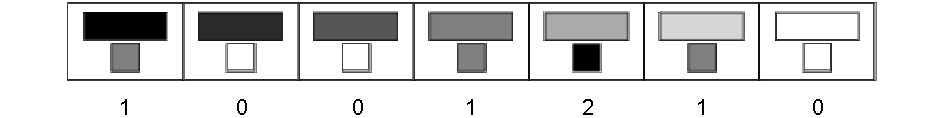
\includegraphics[width=1\textwidth]{fig_totalistcRule777.pdf}
	  \caption{Tabela de transição do AC totalístico 777. As transições dependem da média dos estados das células da vizinhança. Cada média possível é representada por tons de cinza entre o branco (estado 0) e o preto (estado 2).}
	  \label{fig:totalistcRule}
	\end{figure}

Já os ACs semi-totalísticos (\textit{outer-totalistic CA}) são generalizações de ACs totalísticos \cite{weisstein2015outerTotalistic}. Um AC pode ser considerado semi-totalístico caso suas transições sejam definidas pela soma (ou média) das células da vizinhança sem levar em consideração a célula central.

%talvez trocar citação de Gardner.
O Jogo da Vida \cite{GardnerM1970} é o exemplo mais conhecido de autômatos celulares semi-totalísticos, tendo em vista que as células centrais no Jogo da Vida são definidas em termos de ``viva'' (estado 1) ou ``morta'' (estado 0).

Os ACs semi-totalísticos podem ser interpretados como ACs clássicos que apresentam a propriedade de \textit{semi-totalidade}. A propriedade de semi-totalidade determina que as transições que apresentem a mesma soma dos estados vizinhos externos e que tenham a mesma célula central devem apresentar o mesmo resultado. Da mesma forma os ACs totalísticos também tem sua propriedade correspondente nos ACs clássicos: a \textit{totalidade}. A totalidade determina que todas as transições que apresentem a mesma soma dos estados das vizinhanças devem levar a um mesmo resultado.

A partir das definições de como devem ser as transições de estados dos ACs totalísticos e dos ACs semi-totalísticos foi possível representá-los por meio de templates. A biblioteca \textit{CATemplates} já apresenta os algoritmos que geram essas propriedades e seu funcionamento é bem simples. 

O algoritmo que gera regras totalísticas recebe como argumento os valores de $r$ e $k$, definindo assim uma família de ACs. Em seguida enumera as vizinhanças do espaço e calcula a soma dos estados de cada uma delas. O resultado da soma é o que define quais transições devem ser iguais para que o template represente apenas regras totalísticas.

Para determinar qual será a variável associada, dada uma vizinhança qualquer, o algoritmo verifica se a vizinhança foi a única até então que obteve um determinado valor de soma. Em caso positivo o algoritmo criará e associará uma variável $x_i$ para esta transição, sendo $i$ o valor decimal da vizinhança. Caso contrário, a transição será associada uma variável $x_i$ em que $i$ é o valor decimal da primeira e menor vizinhança encontrada com o mesmo valor de soma das vizinhanças.

A Eq. \eqref{eq:templateTotalisticECA} representa o template para o espaço elementar gerado pelo processo descrito acima. Esse template, quando expandido, gera $k^m = 2^4 = 16$ regras.
\begin{equation}
\begin{split}
(x_7,x_3,x_3,x_1,x_3,x_1,x_1,x_0)
\label{eq:templateTotalisticECA}
\end{split}
\end{equation}

Já para a família de ACs de $k=3$ e $r=1$, o algoritmo gera o template demonstrado pela Eq. \eqref{eq:templateTotalistic31}, sendo que esse template representa as $k^m = 3^7 = 2.187$ regras totalísticas do espaço.
\begin{equation}
\begin{split}
(x_{26},x_{17},x_8,x_{17},x_8,x_5,x_8,x_5,x_2,x_{17},x_8,x_5,x_8,\\
x_5,x_2,x_5,x_2,x_1,x_8,x_5,x_2,x_5,x_2,x_1,x_2,x_1,x_0)
\label{eq:templateTotalistic31}
\end{split}
\end{equation}

Para as regras semi-totalísticas, o algoritmo segue o mesmo processo básico, porém com uma pequena modificação: as vizinhanças são somadas, mas a célula central é desconsiderada na soma e posteriormente concatenada ao final do resultado. Neste processo as vizinhanças que contenham o mesmo estado na célula central e a mesma soma de valores dos estados das células externas, como por exemplo $(2,1,0)$ e $(1,1,1)$, geram a mesma cadeias de caracteres ao final. A partir desse ponto o algoritmo segue a mesmo processo aplicado as regras totalísticas: para determinar qual será a variável associada a uma vizinhança o algoritmo verifica se a vizinhança foi a única até então que obteve um determinado valor. Em caso positivo o algoritmo criará e associará uma variável $x_i$ para esta transição, sendo $i$ o valor decimal da vizinhança. Caso contrário, a transição será associada uma variável $x_i$ em que $i$ é o valor decimal da primeira e menor vizinhança encontrada com o mesmo valor de soma das vizinhanças.

Aplicando esse algoritmo gerador de templates de regras semi-totalísticas como os argumentos $k=2$ e $r=1$ é obtido o template representado pela Eq. \eqref{eq:templateSemiTotalisticECA}.
\begin{equation}
\begin{split}
(x_7,x_3,x_5,x_1,x_3,x_2,x_1,x_0)
\label{eq:templateSemiTotalisticECA}
\end{split}
\end{equation}

O template representado pela Eq. \eqref{eq:templateSemiTotalisticECA} quando expandido gera as $k^m = 2^6 = 64$ regras semi-totalísticas do espaço elementar.

Para a família de ACs com $k=3$ e $r=1$, o algoritmo gera o template representado pela Eq. \eqref{eq:templateSemiTotalistic31}, que quando expandida gera as $k^m = 3^{15} = 14.348.907$ regras semi-totalísticas do espaço.
\begin{equation}
\begin{split}
(x_{26},x_{17},x_8,x_{23},x_{14},x_5,x_{20},x_{11},x_2,x_{17},x_8,x_7,x_{14},\\
x_5,x_4,x_{11},x_2,x_1,x_8,x_7,x_6,x_5,x_4,x_3,x_2,x_1,x_0)
\label{eq:templateSemiTotalistic31}
\end{split}
\end{equation}

%!TEX root = dissertacao.tex
\section{DIFERENÇA ENTRE TEMPLATES}
\label{sec:resultadosParciais}
Este capítulo apresenta o desenvolvimento da operação de diferença entre templates com $k=2$, introduz-se a operação de geração de templates de exceção, e demonstra-se uma série de passos que, utilizando templates, pode auxiliar na busca de ACs de raio 3 que tem a possibilidade de solucionar o problema de paridade.

\subsection{Templates de Exceção}
Alguns templates apresentam em seus campos valores que, quando expandidos, gerarão substituições inválidas e, por consequência, regras inválidas. O template $T_o = (x_7, x_6, x_5, 1 - x_1 - x_5, 2 - x_1 - x_2, x_2, x_1, 0)$ com $k=2$ é um exemplo disso. É trivial perceber que qualquer expansão do template $T_o$ que tenha o conjunto de substituições $\{x_1 = 1, x_5 = 1\}$ fará com que a posição 4 do template apresente o valor $2$, que não pertence ao intervalo $[0,k-1]$; da mesma maneira, qualquer expansão do template $T_o$ que tenha o conjunto de substituições $\{x_1 = 0, x_2 = 0\}$ fará com que a posição 3 do template também apresente um valor que não pertence ao intervalo $[0,k-1]$. Um \textit{template de exceção} é um template que apresenta esses conjuntos substituições que levam um template passado com parâmetro a apresentar substituições fora do intervalo inteiro $[0, k-1]$. Já o conjunto de \textit{template de exceção} de um template representa todas os templates de exceção encontrados apartir do template passado como parâmetro. O conjunto de templates de exceção do template $T_o$, utilizado como exemplo, pode ser representado pela Eq. \ref{eq:exceptionsTemplates}.

\begin{equation}
C_e = \{(x_7, x_6, 1, x_4, x_3, 1, x_2, x_0),(x_7, x_6, x_5, x_4, x_3, 0, 0, x_0)\}
\label{eq:exceptionsTemplates}
\end{equation}

Formalmente, a operação geradora de templates de exceção $X$ gera um conjunto $C_e$ com todos os templates de exceção do template $T_o$ passado como parâmetro. A operação que gera o conjunto templates de exceção de um template pode ser descrita em mais detalhes da seguinte maneira:
\begin{equation}
\begin{split}
X(T_o)= C_e \\
C_e = \{T_1,T_2,\dots, T_n\}\\
\end{split}
\end{equation}

O algoritmo dessa operação primeiro encontra todas as posições que não apresentem apenas variáveis livres ou constantes. Geram então para cada uma das posições encontradas todas as substituições possíveis, dentro do intervalo $[0,k-1]$, para cada uma das variáveis presentes na posição. Por fim, verifica se a solução com as substituições possíveis levam valores fora dos intervalos $[0,k-1]$.

Para exemplificar, considere o template $T_{o} = (1, x_6, x_5, 1 - x_1 - x_2, 2 - x_1 - x_2, x_2, x_1, 0)$. O primeiro passo do algoritmo é encontrar um conjunto com as posições que não apresentem apenas constantes ou variáveis livres, obtendo-se assim $\{\{1 - x_1 - x_2\}, \{2 - x_1 - x_2\}\}$. Então, aplica-se à cada um dos itens do conjunto obtido todas as combinações possíveis das substituições de $x_1$ e $x_2$, conforme mostrado na Tabela \ref{tab:exceptionProcessA} e \ref{tab:exceptionProcessB} para $\{\{1 - x_1 - x_2\}, \{2 - x_1 - x_2\}\}$ respectivamente.
\begin{table}[h!]
\centering
\caption{Expansão do campo 1 - x_1 - x_2.}
	\begin{tabular}{ccc}
    \toprule
	$x_2$ & $x_1$ & Expansão do campo \\
    \midrule
	0	&	0	&	1 - x_1 - x_2 = 1	\\
	0	&	1	&	1 - x_1 - x_2 = 0	\\
	1	&	0	&	1 - x_1 - x_2 = 0	\\
	1	&	1	&	1 - x_1 - x_2 = -1	\\
    \bottomrule
	\end{tabular}
\label{tab:exceptionProcessA}
\end{table} 

\begin{table}[h!]
\centering
\caption{Expansão do campo 2 - x_1 - x_2.}
	\begin{tabular}{ccc}
    \toprule
	$x_2$ & $x_1$ & Expansão do campo \\
    \midrule
	0	&	0	&	2 - x_1 - x_2 = 2	\\
	0	&	1	&	2 - x_1 - x_2 = 1	\\
	1	&	0	&	2 - x_1 - x_2 = 1	\\
	1	&	1	&	2 - x_1 - x_2 = 0	\\
    \bottomrule
	\end{tabular}
\label{tab:exceptionProcessB}
\end{table}

Para finalizar a operação, o algoritmo seleciona as substituições que geram valores inválidos, e aplicam ela ao template base, gerando assim o conjunto de templates $C_e$, mostrado na  Eq. \ref{eq:exceptionsTemplates2}.

\begin{equation}
C_e = \{(x_7, x_6, x_5, x_4, x_3, 1, 1, x_0),(x_7, x_6, x_5, x_4, x_3, 0, 0, x_0)\}
\label{eq:exceptionsTemplates2}
\end{equation}

A operação que gera os templates de exceção foi apresentada por Soares, Verardo e
de Oliveira (\citeyear{soares2016difference}) e é importante por ser essencial para a operação de diferença entre templates. 

É importante frisar que essa é uma operação com complexidade $O(c^n)$, onde $n$ é o número de variáveis nas posições que não apresentem apenas variáveis livres ou constantes. Por conta disso, a operação de diferença pode se mostrar demasiadamente custosa quando aplicadas a templates com muita dependências entre variáveis, tais como os templates de conservabilidade e conservabilidade de paridade.

\subsection{Diferença entre Templates binários}
A operação de diferença $D_i$ entre templates binários é responsável por obter um conjunto $C_{di}$ com $n$ templates, os quais, quando expandidos (via a operação de expansão $E$), apresentam apenas as regras geradas pela expansão do template $T_m$ que não estejam também presentes na expansão do template de intersecção entre $T_s$ e $T_m$, chamado aqui de $T_i$. A operação de diferença pode ser descrita em mais detalhes da seguinte maneira:
\begin{equation}
\begin{split}
D_i(T_m,T_s)= C_{di} \Leftrightarrow E(C_{di}) = E(T_m) \setminus E(T_i) \\
T_i = I(T_m,T_s)\\
C_{di} = \{T_1,T_2,\dots, T_n\}\\
\end{split}
\end{equation}

A Figura \ref{fig:complement} ilustra essa operação, onde os templates $T_m$ e $T_s$ passados como parâmetro para a operação de diferença estão representado pelos dois círculos, e o conjunto $C_{di}$ retornado pela função está representado pela área em cinza na imagem.
\begin{figure}[h!]
  \centering
  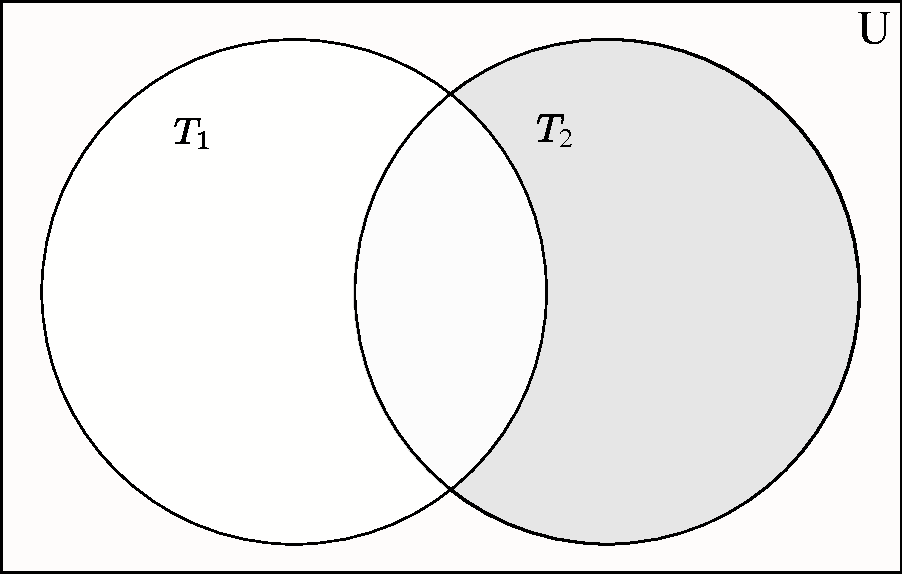
\includegraphics[width=.4\textwidth]{fig_complement2.pdf}
  \caption{Os círculos $T_m$ e $T_s$ são os templates que representam dois conjuntos de regras. Em cinza, $C_{di}$ é o conjunto de templates que representam o conjunto de regras retornado pela operação de diferença entre $T_m$ e $T_s$.}
  \label{fig:complement}
\end{figure}    

O processo que o algoritmo usa para encontrar a diferença entre dois templates é efetuado através de uma sequência de etapas. A primeira etapa consiste em encontrar o template $T_i$, que é a intersecção entre os templates $T_m$ e $T_s$, ambos recebidos como parâmetro. Em seguida, igualam-se os templates $T_m$ e $T_i$, obtendo-se assim combinações lógicas de equações. Após remover eventuais equações tautológicas, o algoritmo aplica a operação de negação nas equações e troca o operador lógico $\wedge$ por $\vee$, que, no caso binário, consistem apenas em efetuar as permutações $\rho = (0 \rightarrow 1, 1 \rightarrow 0, \wedge \rightarrow \vee)$ ao resultado final das equações. Esse sistema é então solucionado, resultando num conjunto com diversos conjuntos de regras de substituições, as quais são aplicadas ao template $T_i$, gerando um conjunto de templates que é parte do resultado dessa operação. Um segundo conjunto de templates será a outra parte do resultado. Esse conjunto será gerado a partir da intersecção de cada um dos templates de exceção do template $T_i$ com o template $T_m$.

Para melhor visualizar essas etapas, considerem-se os templates $T_m = (x_7, x_6, x_5, x_4, x_3, x_1, x_1, x_0)$ e $T_s = (x_7, x_6, x_3 + x_1, 1 - x_1, x_3, x_1, x_1, 0)$, ambos com $k=2$ e $r=1$. Esses templates serão primeiramente passados para a operação de intersecção, gerando assim o template $T_i = (x_7, x_6, x_3 + x_1, 1 - x_1, x_3, x_1, x_1, 0)$. Na sequência, igualam-se os templates $T_m$ e $T_i$, o que gera o sistema de equações mostrado na Eq. \eqref{eq:complement}.
\begin{equation}
\left\{\begin{matrix}
x_7 & = & x_7	\\ 
x_6 & = & x_6	\\ 
x_5 & = & x_3 + x_1	\\ 
x_4 & = & 1 - x_1 \\ 
x_3 & = & x_3	\\ 
x_1 & = & x_1	\\ 
x_1 & = & x_1	\\ 
x_0 & = & 0
\end{matrix}\right.
\label{eq:complement}
\end{equation}

Esse sistema deve ser representado através de combinações lógicas de equações, como se pode ver na Eq. \eqref{eq:logicalComplement}, que é equivalente à Eq. \eqref{eq:complement}.
\begin{equation}
\begin{split}
x_7 = x_7	\wedge  
x_6 = x_6	\wedge  
x_5 = x_3 + x_1	\wedge  
x_4 =   1 - x_1 \wedge  \\
x_3 = x_3	\wedge  
x_1 = x_1	\wedge  
x_1 = x_1	\wedge  
x_0 = 0
\end{split}
\label{eq:logicalComplement}
\end{equation}

Antes de solucionar a Eq. \eqref{eq:logicalComplement}, o algoritmo elimina todas as equações tautológicas e troca todo operador lógico $\wedge$ por $\vee$; como resultado, obtêm-se a Eq. \eqref{eq:logicalComplement1}.
\begin{equation}
x_5 = x_3 + x_1 \vee x_4 = 1 - x_1 \vee x_0 = 0
\label{eq:logicalComplement1}
\end{equation}

Por fim,  aplica-se a operação de negação nas equações. No caso binário basta efetuar a permutação $\rho$, que também pode ser feita por meio da função $f(x) = 1 - x$. A Eq. \eqref{eq:logicalComplement2} representa a combinação lógica de equações que resulta das operações precedentes.
\begin{equation}
x_5 = 1 - (x_3 + x_1) \vee x_4 = 1 - (1 - x_1) \vee x_0 = 1 - 0
\label{eq:logicalComplement2}
\end{equation}

A combinação lógica de equações é então solucionada, resultando no conjunto solução $S = \{\{x_0 \to 1\}, \{x_4 \to x_1\}, \{x_5 \to 1 - x_1 - x_3\}\}$. Perceba-se que $S$ apresenta mais de um conjunto de substituições e, portanto, cada um deles deve ser utilizado para realizar as substituições no template $T_m$. Essas substituições fazem com que se obtenha o conjunto de templates $C_{d1}$, representados pela Eq. \eqref{eq:logicalComplement3}. 
\begin{equation}
\begin{split}
C_{d1} = \{\\(x_7, x_6, x_5, x_4, x_3, x_1, x_1, 1), \\(x_7, x_6, x_5, x_1, x_3, x_1, x_1, x_0), \\(x_7, x_6, 1 - x_1 - x_3, x_4, x_3, x_1, x_1, x_0)\\\}
\end{split}
\label{eq:logicalComplement3}
\end{equation}

Os templates do conjunto $C_{d1}$ farão parte do conjunto $C_{di}$ resultante da operação de diferença. Entretanto, é necessário verificar se o template $T_i$ possui combinações de substituições que o levem a gerar regras inválidas. Isso é feito passando o template $T_i$ para a operação geradora de template de exceção, o que resulta no conjunto de templates $\{(x_7, x_6, x_5, x_4, 1, x_2, 1, x_0)\}$ (que, no caso, só possui 1 elemento). Os templates desse conjunto são então interseccionados com o template $T_m$, resultando no conjunto $C_e = \{(x_7, x_6, x_5, x_4, 1, 1, 1, x_0)\}$. Por fim, faz-se a unificação dos conjuntos $C_{d1}$ e $C_e$, obtendo-se o conjunto de templates $C_{di}$, representado pela Eq. \ref{eq:complementionSet}.
\begin{equation}
\begin{split}
C_{d1} = \{\\(x_7, x_6, x_5, x_4, x_3, x_1, x_1, 1), \\(x_7, x_6, x_5, x_1, x_3, x_1, x_1, x_0), \\(x_7, x_6, 1 - x_1 - x_3, x_4, x_3, x_1, x_1, x_0), \\(x_7, x_6, x_5, x_4, 1, 1, 1, x_0)\\\}
\label{eq:complementionSet}
\end{split}
\end{equation}

A operação de diferença $D_i$ também pode ser realizada sem se efetuar se realizar a intersecção. Nesse caso, a operação sem intersecção chamada aqui apenas apenas por $D$, encontrará um conjunto de templates $C_d$. A expansão dos templates de $C_{d}$ apresentará apenas as regras geradas pela expansão do template $T_m$ que não estejam também presentes na expansão do template $T_s$. Essa operação pode ser descrita em mais detalhes da seguinte maneira:
\begin{equation}
\begin{split}
D(T_m,T_s)= C_d \Leftrightarrow E(C_d) = E(T_m) \setminus E(T_s) \\
C_d = \{T_1,T_2,\dots, T_n\}\\
\end{split}
\end{equation}

O processo que o algoritmo da operação $D$ usa para encontrar a diferença entre dois templates é bem parecido com o do algoritmo da operação $D_{i}$. Primeiramente, igualam-se os templates $T_m$ e $T_s$, obtendo-se assim combinações lógicas de equações. Após remover eventuais equações tautológicas, o algoritmo aplica a operação de negação nas equações e troca o operador lógico $\wedge$ por $\vee$. Esse sistema é então solucionado, resultando num conjunto com diversos conjuntos de regras de substituições. E após eliminar desse conjunto eventuais substituições envolvendo variáveis que não pertençam ao $T_m$, esses conjuntos de regras de substituição são aplicados ao template $T_m$, gerando o conjunto de templates que é parte do resultado dessa operação. Um segundo conjunto de templates, composto pela intersecção de cada um dos templates de exceção do template $T_s$ com o template $T_m$, será a outra parte do resultado.

Os algortimos $D$ e $D_i$ apresentam como resultado os conjunto de templates $C_d$ e $C_{di}$, respectivamente. $C_d$ e $C_{di}$ podem ser diferentes mesmo quando $D$ e $D_i$ recebem os mesmos templates como entrada. Mas ambos contém exatamente as mesmas regras quando se expande os templates dos conjuntos.

A implementação das operações de diferença foi desenvolvida na linguagem do software \textit{Wolfram Mathematica} \cite{woframMathematica10} e na mesma linguagem foram criados os testes unitários que verificam se o \textit{output} da operação está correto de acordo com os possíveis \textit{input} dados a ela. Todos os testes receberam dois templates, $T_m$ e $T_s$, expandiram esses dois templates individualmente, e depois subtraíram das regras encontradas na expansão de $T_m$ todas as regras representadas por $T_s$. O resultado da diferença entre $T_m$ e $T_s$ é o conjunto de regras $C_{exp}$. Esse conjunto de regras $C_{exp}$ deve ser idêntico às regras geradas pela expansão dos templates resultantes da operação de diferença entre os templates $T_m$ e $T_s$. Por conta desta custosa forma de teste, os testes dessa operação se concentraram nos raios 1, 2 e 3.

\section{DISCUSSÃO E TESTES}
\label{sec:discussoesETestes}
Uma importante questão sobre a expansão do conjunto de regras $C_{exp}$ encontrado pela operação de diferença é definir qual será o pós-processamento da operação de expansão que deve ser usado com esses templates. A operação de pós-processamento a ser utilizada na operação de diferença sempre será a mesma utilizada no template $T_m$ passado como parâmetro, acrescida da operação de filtro das regras inválidas, caso essa operação já não tenha sido feita. Isto porque a operação de diferença deve representar todas as regras válidas da expansão de $T_m$ que não sejam representadas por $T_s$. Assim, caso $T_m$ e $T_s$ não tenham intersecção, o resultado deve ser apenas o template $T_m$ com o mesmo pós-processamento.



Nos testes para todos os raios foi gerado um conjunto de templates e, a partir dele, geraram-se todos os pares de combinações possíveis. Por fim, foi realizado o teste da operação de diferença com cada um dos pares de template gerados.

Para os testes com $r = 1$, cada um dos templates do conjunto usado para os testes representava uma das seguintes propriedades estáticas: conservabilidade de estados; confinamento; totalidade; semi-totalidade; e invariância  à troca de cor. Além desse templates, também foi utilizado o template base, que representa todas as regras do espaço.

Para os testes com $r = 2$, os templates usados representavam as seguintes propriedades estáticas: Conservabilidade de estados; totalidade; semi-totalidade; e invariância à troca de cor. Já para os testes $r = 3$, os templates de teste representavam apenas as propriedades estáticas de totalidade e semi-totalidade. Foram feitos testes com menos propriedades de acordo com o raio pois esses testes envolvem expansões, que para algumas dessas propriedades consiste em enumerar um número muito grande de regras. Assim os testes foram feitos apenas com propriedades em que a expansão dos templates encontrados consista em enumerar menos que $2^{16}$ regras. A Tabela \ref{tab:differenceTests} mostra em mais detalhes os templates de quais propriedades estáticas foram testados em cada raio.

\begin{table}[h!]
\centering
\caption{Teste de diferença entre templates feito em cada raio}
\resizebox{\textwidth}{!}{%
\begin{tabular}{l|lllll|}
\cline{2-6}
& \multicolumn{5}{c|}{Template minuendo ($T_m$)} \\ \cline{1-1}
\multicolumn{1}{|l|}{Template subtraendo ($T_s$)}                  
& totalidade
& semi-totalidade
& \begin{tabular}[c]{@{}l@{}}conservabilidade\\ de estados\end{tabular} 
& \begin{tabular}[c]{@{}l@{}}invariância à\\ troca de cor\end{tabular}  
& confinamento 
\\ \cline{2-6} 

\multicolumn{1}{|l|}{totalidade} 				  & Raio 1, 2 e 3& Raio 1, 2 e 3  & Raio 1 e 2& Raio 1 e 2& Raio 1	\\
\multicolumn{1}{|l|}{semi-totalidade} 			  & Raio 1, 2 e 3& Raio 1, 2 e 3  & Raio 1 e 2& Raio 1 e 2& Raio 1	\\
\multicolumn{1}{|l|}{conservabilidade de estados} & Raio 1 e 2	 & Raio 1 e 2	  & Raio 1 e 2& Raio 1 e 2& Raio 1	\\
\multicolumn{1}{|l|}{invariância  à troca de cor} & Raio 1 e 2	 & Raio 1 e 2	  & Raio 1 e 2& Raio 1 e 2& Raio 1	\\
\multicolumn{1}{|l|}{confinamento}                & Raio 1		 & Raio 1		  & Raio 1	& Raio 1	& Raio 1	\\ \hline
\bottomrule
\end{tabular}%
}
\label{tab:differenceTests}
\end{table}

Ademais, esses testes mostraram que a operação de diferença está funcionando para diversos templates, sem a necessidade de operações específicas para cadas uma deles.

É importante explicitar que a implementação do algoritmo que executa a operação de diferença entre templates ainda não permite trabalhar com $k\neq 2$, pois a negação das equações são feitas por meio da função $f(x) = 1 - x$.

\subsection{Templates aplicados no problema de paridade}
O desenvolvimento da operação de diferença entre template permite diversas possibilidades de aplicação.
Uma possibilidade que foi aventada é no problema de paridade. 
Ainda não se sabe se existem regras de raio 3 que solucionem o problema de paridade \cite{Betel2013}. 
Mas o uso de templates e suas operações podem ser uma forma interessante de restringir o conjunto de regras na busca dessa solução.

As regras dos ACs que solucionam o problema de paridade têm algumas propriedades estáticas que podem ser trivialmente percebidas. 
Um AC que resolva o problema de paridade sempre será confinado, tendo em vista que as vizinhanças homogêneas não devem levar a transições de estado ativas, a qual é a única restrição de variável nos templates confinados para AC binários. 
O espaço das regras confinadas de raio 3 ainda é muito grande; entretanto, essa não é a única propriedade estática que um AC que resolva o problema de paridade apresenta.  Nesse sentido, também é necessário que ele não seja conservativo, visto que, se a soma dos estados do AC não mudar, ele nunca convergirá como propõe o problema. 
Por fim, espera-se que um AC que resolva o problema de paridade seja conservativo de paridade.

Dada a possibilidade de se obter os templates para todas essas propriedades, é também possível utilizar esses templates e as operações de diferença e intersecção para expressar esse espaço de busca para a solução do problema de paridade.
Para efetuar esta expressar esse espaço, basta efetuar a intersecção dos templates de confinamento com o template de conservabilidade de paridade, visto que ambas as propriedades são necessárias. Entretanto, vale frisar que essa intersecção gera o próprio template de paridade, não fazendo diferença para o resultado final.
Posteriormente, deve-se efetuar a operação de diferença com o template obtido pela primeira intersecção com o template das regras conservativas de estado, já que as conservabilidade de estado impede a resolução do problema de paridade.

Formalmente, essas operações de conjuntos entre os templates podem ser representadas através da Eq. \eqref{eq:operationsTemplateParidade}, sendo que $T_{confinado}$ representa o template das regras confinadas, $T_{conservaparidade}$ representa o templates das regras que conservam a paridade, e ${T}_{conservaestados}$ indica o template de regras conservativas. O resultado dessa operação é $T_{paridade}$, o qual representa um conjunto de templates que restringem um pouco mais as regras com possibilidades de solucionar o problema de paridade.
\begin{equation}
T_{paridade} = (T_{conservaparidade} \cap T_{confinado}) - {T}_{conservaestados}
\label{eq:operationsTemplateParidade}
\end{equation}

Entretanto, apesar de formalmente possível, a realização dessas operações não se mostraram produtivas. Isto ocorre pois  a operação de exceção, utilizada pela operação de diferença, tem complexidade $O(c^n)$, onde $n$ é o número de variáveis nas posições que não apresentem apenas variáveis livres ou constantes. Deste modo, gerar os templates de exceção do template $T_{conservaestados}$ é tão custoso quanto expandir todas as regras desse template.

Dito isto, é mais simples utilizar o template $T_{conservaestados}$ com uma função de pós-processamento alternativa que elimine todas as tabelas $k$-árias que não apresentem campos inválidos, e aplique $mod$ $2$ nas restantes. Assim  esse mesmo template vai representar apenas as regras que mantenham a paridade mas não apresentem a propriedade de conservabilidade de estados. Também poderá ser aplicado nesse template operações de intersecção ou diferença com outros templates de modo a se restringir ainda mais o espaço de busca.

%!TEX root = dissertacao.tex
\section{CONSIDERAÇÕES FINAIS}
\label{sec:consideracoesFinais}

No presente trabalho são descritos os templates de autômatos celulares unidimensionais, proposta introduzida por de Oliveira e Verardo (\citeyear{deOliveira2014}), que, por meio de uma generalização de suas tabelas de transição $k$-árias, pode representar conjuntos de regras que compartilham determinadas propriedades.

Essa capacidade faz com que não seja necessário buscar ACs com essas propriedades por todo um espaço, o que impossibilitaria a busca através de força bruta, devido ao rápido crescimento das famílias dos ACs conforme se mudam seus parâmetros. Adicionalmente, mesmo buscas heurísticas também ficam facilitadas no sub-espaço definido pelos templates.

Por conta dessa capacidade de representação de ACs com determinadas propriedades, foram descritos aqui algumas propriedades estáticas e os algoritmos geradores dos templates que as representam. Esses algoritmos já estavam implementados na biblioteca \textit{open source} \textit{CATemplates} \cite{CATemplates}. Além disso, foram explicadas as operações de expansão e intersecção do \textit{CATemplates}. Essas operações, desenvolvidas por \citeonline{Verardo2014}, foram mostradas novamente aqui para que fosse possível explicitar sua relevância para a solução de problemas típicos de ACs, como o problema de paridade.

Também apresentamos a operação de diferença entre templates e a operação geradora de templates de exceção, ambas introduzidas por Soares, Verardo e de Oliveira (\citeyear{soares2016difference}). A operação de diferença entre templates permite que se encontre um conjunto de templates que represente todas as regras que não pertençam ao template passado como argumento. Esta operação -- que no momento só aceita templates binários -- já está disponível na biblioteca \textit{CATemplates}, e é mais um exemplo de operação que pode ser utilizada para restringir o conjunto de regras a serem avaliadas na busca pela solução de algum problema.

Para que fosse possível a implementação da operação de diferença, foi desenvolvida a operação que, dado um template, gera os \textit{templates de exceção} correspondentes. \textit{Templates de exceção} são gerados a partir de templates base, substituindo-se algumas variáveis pelas substituições que geram regras inválidas no template original. O algoritmo que gera templates de exceção é essencial para a operação de diferença.

Também foi exposto nesse trabalho um conjunto de processos utilizando templates que podem auxiliar na restrição do espaço de busca para a solução do problema de paridade.

Como possíveis trabalhos futuros, pretende-se generalizar a operação de diferença para qualquer valor de $k$, bem como pretende-se implementar novos algoritmos geradores de templates que representem outras propriedades estáticas. Ademais, pode-se buscar também a implementação de novas operações de templates baseadas nas operações de conjuntos, como a operação de união de templates.


%!TEX root = qualificacao.tex
\section{PLANO DE TRABALHO}
\label{sec:planoDeTrabalho}

Este projeto está organizado em sete fases, em um período de dois anos, conforme descrito na tabela \ref{cronograma}:

  \begin{itemize}
      \item Fase 0: participação nas disciplinas necessárias ao cumprimento dos créditos para a obtenção do título de mestre;
      \item Fase 1: pesquisa bibliográfica de autômatos celulares e de templates;
      \item Fase 2: programação e testes da operação de complemento de templates e de operações de geração de templates de exceção;
      \item Fase 3: proposição de propriedades estáticas para se gerar templates;
      \item Fase 4: programação e testes de operações de geração de templates;
      \item Fase 5: submissão de artigo;
      \item Fase 6: escrita da dissertação.
  \end{itemize}

\begin{table}[h!]
\centering
\caption{Cronograma de desenvolvimento do projeto}
\label{cronograma}
\resizebox{\textwidth}{!}{
	\vspace{0cm}
	\begin{tabular}{|l|c|c|c|c|c|c|c|c|}
	\hline	
	\multicolumn{1}{|c|}{} 	& \multicolumn{4}{c|}{2014} 					& \multicolumn{4}{c|}{2015}						\\ \hline
	\textbf{Atividades} 	& Jan-Mar	& Abr-Jun 	& Jul-Set 	& Out-Dez	& Jan-Mar	& Abr-Jun 	& Jul-Set 	& Out-Dez	\\ \hline
	Fase 0 					&  •		& •			& •			& •			&   		& •			&  			&  			\\ \hline
	Fase 1				 	&   		&  			&  			& •			&  •		& 			&  			&  			\\ \hline
	Fase 2				 	&   		&  			&  			& 			&  •		& •			&  			&  			\\ \hline
	Fase 3				 	&   		&  			&  			&  			&   		&  			& •			& 			\\ \hline
	Fase 4				 	&   		&  			&  			&  			&   		&  			& •			& •			\\ \hline
	Fase 5				 	&   		&  			&  			&  			&   		&  			& •			&  			\\ \hline
	Fase 6				 	&   		&  			&  			&  			&   		& •			& •			& •			\\ \hline
	\hline
	\end{tabular}
}
\end{table}

\def\refname{REFERÊNCIAS BIBLIOGRÁFICAS}
\bibliography{bibliografia}
\addcontentsline{toc}{section}{REFERÊNCIAS BIBLIOGRÁFICAS} 
\bibliographystyle{abnt-alf}

\end{document}
